\documentclass[aspectratio=169]{beamer}
\usepackage{ctex, hyperref}
\usepackage{calligra}
\usepackage[T1]{fontenc}
\author{Heran Zhu}
\title{Robust AI Project Team}
\subtitle{Weekly Report}
\institute{Electronic Information School, Wuhan University}
\date{Oct 9th, 2021}
\usepackage{WHU}

\usepackage{tcolorbox}

% \usepackage{graphicx}
% \usepackage{caption2}
\usepackage{subfigure}
% \usepackage{float}
\usepackage{wrapfig}	% 图文混排
\usepackage{multicol}	% 多列
\usepackage{mathrsfs}	% 花体数学
\usepackage{amsmath,amsthm,amsfonts,amssymb,bm}


\usepackage[backend=bibtex,sorting=none]{biblatex}
\addbibresource{ref.bib} %BibTeX数据文件及位置
\setbeamerfont{footnote}{size=\tiny}
\begin{document}

\kaishu
\begin{frame}
	\titlepage
	\begin{figure}[htb]
		\begin{center}
			
\includegraphics[width=0.1\linewidth]{pic/whulogo.eps}
		\end{center}
	\end{figure}
\end{frame}

% \begin{frame}
% \tableofcontents[sectionstyle=show,subsectionstyle=show/shaded/hide,subsubsectionstyle=show/shaded/hide]
% \end{frame}


% \renewcommand{\thefootnote}{\fnsymbol{footnote}} %不用数字脚注

% ----------------------------------------
% 	--- Paper Reading ---
% ----------------------------------------
% Weakly Supervised Fine-grained Image Classification via 
% 			   Correlation-guided Discriminative Learning
% 基于相关引导判别学习的弱监督细粒度图像分类
% Correlation-guided Discriminative Learning (CDL) model
% \section{Paper Reading: CDL}

\begin{frame}{Weakly Supervised Fine-grained Image Classification via Correlation-guided Discriminative Learning}
    \begin{itemize}
        \item \textbf{Author:} Zhihui Wang, Shijie Wang, Pengbo Zhang...\footnote{大连理工大学王智慧教授、李豪杰教授、王世杰博士等}
        \item \textbf{Keywords:} Fine-grained Image Classification; Discriminative Region Grouping; Discriminative Feature Strengthening
        \footnote{细粒度图像分类,判别区域分组,判别特征增强}
        \item \textbf{Contribution:} \textbf{Propose} an end-to-end Correlation-guided Discriminative Learning (CDL) model to fully mine and exploit the discriminative potentials of correlations for WFGIC globally and locally. 
        \footnote{提出了一个端到端相关性引导判别学习(CDL)模型,以充分挖掘和利用相关性在全局和局部的鉴别潜力。}
        % \item 开源代码:无
    \end{itemize}
\end{frame}

\begin{frame}{Motivation for correlation-guided discriminative learning}
    \begin{figure}[htb]
        \centering
        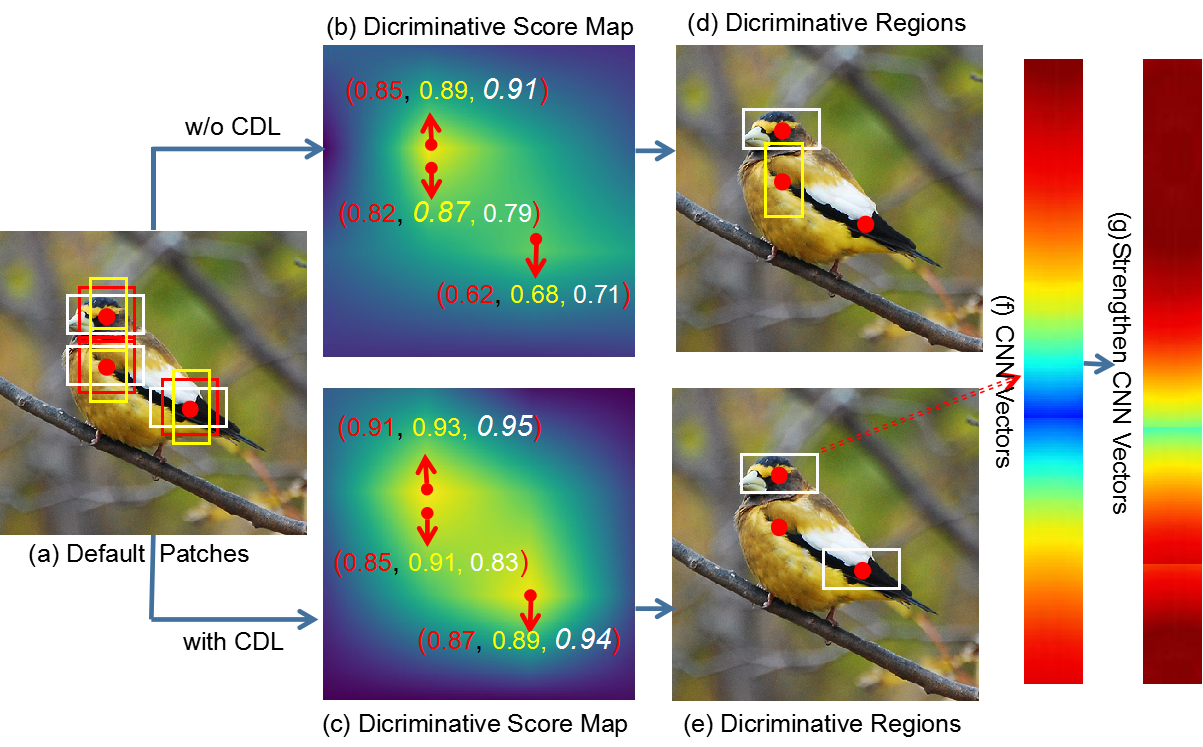
\includegraphics[width=0.6\textwidth]{docs/paperReading/CDL/summary.png}
    \end{figure}
    \begin{scriptsize}
        (b)(d)是没有相关性引导的判别学习,(c)(e)是有相关性引导的判别学习
        
        (f)是CNN的feature,(g)是挖掘相互依赖之后的feature
    \end{scriptsize}
\end{frame}



\begin{frame}{The framework of the Correlation-guided Discriminative Learning (CDL) model}
    \begin{wrapfigure}{l}{0.7\textwidth}    % 靠文字内容的左侧
        \centering
        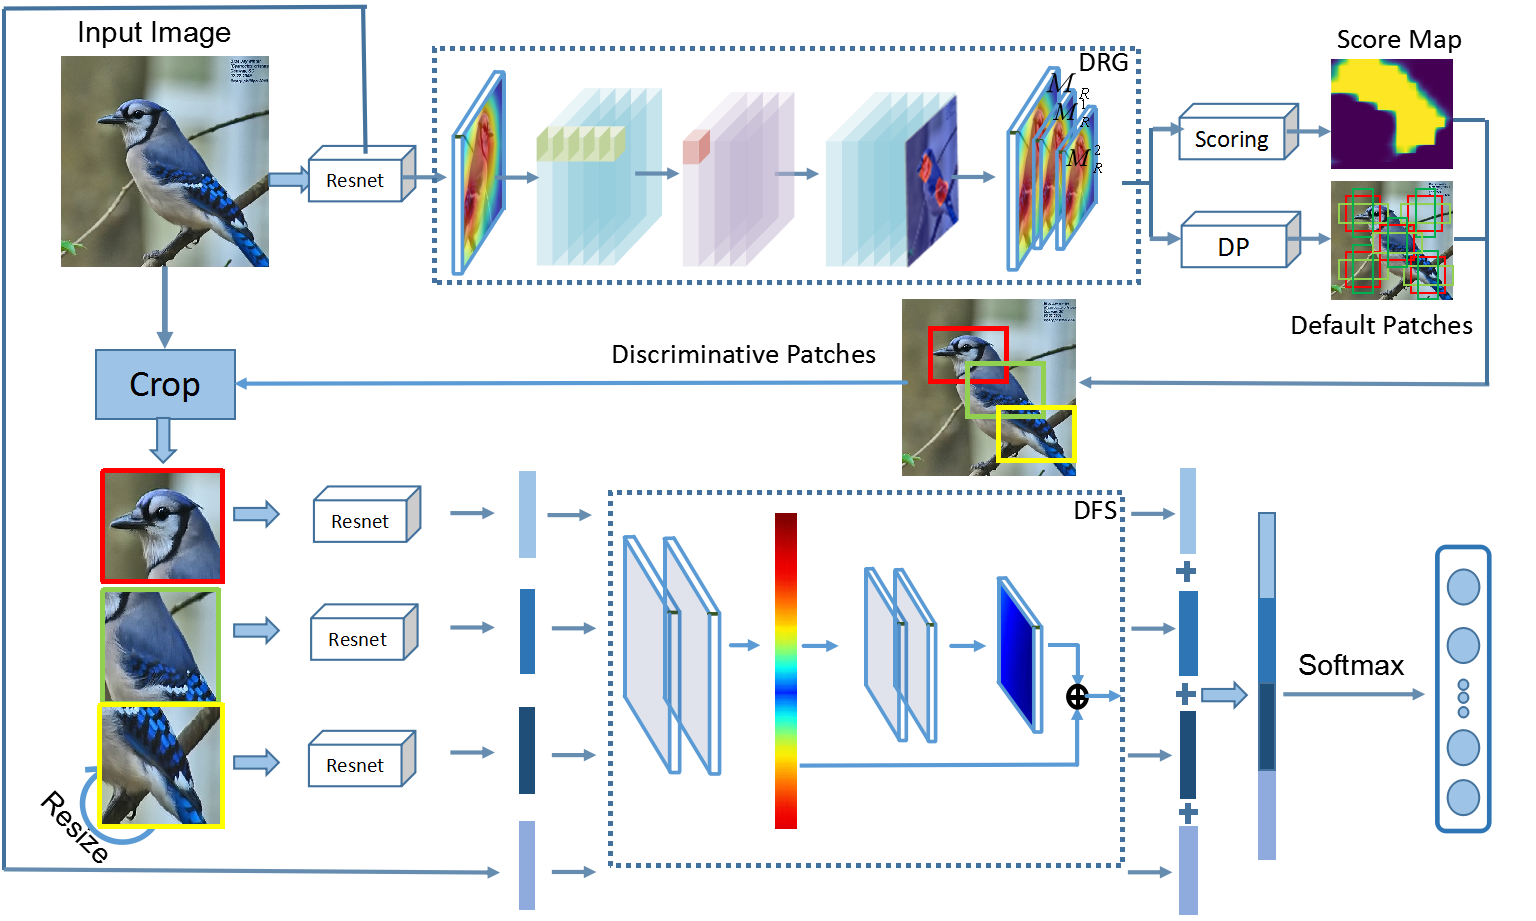
\includegraphics[width=0.6\textwidth]{docs/paperReading/CDL/framework.png}
        % \caption{\footnotesize framework of CDL}
    \end{wrapfigure}

    % 不能在任何列表环境中使用 wrapfigure,也不能在列表环境前后使用,除非两者之间有一空行或分段指令 \par。
    CDL model:
    \begin{scriptsize}
        \begin{itemize}
            \item \textbf{DGR} 判别区域分组子网络
            \item \textbf{Scoring} 评分网络
            \item \textbf{DP} 根据score map选择更具判别性的patch
            \item \textbf{Resize} 224*224
            \item \textbf{DFS}(discriminative feature strengthening) 判别性特征增强子网络
            \item concat the multiply feature
        \end{itemize}
    \end{scriptsize}    
\end{frame}


\begin{frame}{Discriminative Region Grouping(DRG)}
    \begin{multicols}{2}
        \begin{figure}
            \centering
            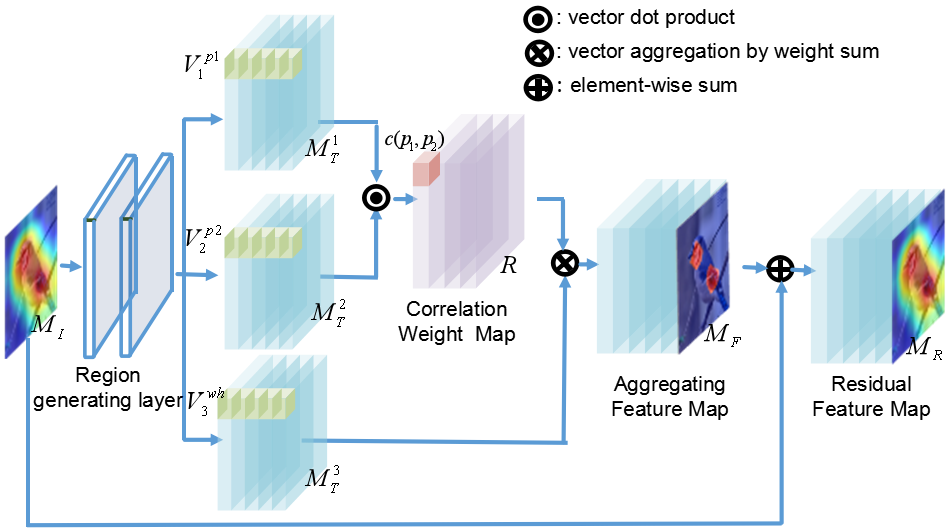
\includegraphics[width=0.52\textwidth]{docs/paperReading/CDL/dgr.png}
        \end{figure}
        
        DRG
        \begin{scriptsize}
            (Discriminative Region Grouping),学习两个区域的相关性系数,与原特征图加权后可以得到聚合特征图,最后通过残差学习将输入特征图的全局语义信息和局部细节信息进行整合,提取出有区别的小块
            \begin{enumerate}
                \item \textbf{region generating layer.}: 1*1 kernel的小区域检测器(small region detector)。
                \item \textbf{correlation layer.}
                \item \begin{equation}
                    R=softmax(V_1^{p_1}\cdot V_2^{p_2})
                \end{equation}
                \item \textbf{fusion(aggregating) layer.}
                \begin{equation}
                    M_F^{ij}=\sum_{w=1}^W\sum_{h=1}^H(V_3^{wh}\cdot R^{ijk}),k=(w-1)\times W+h
                \end{equation}
                \item \textbf{residual block.} $W_R=\alpha\cdot M_F+M_I$
            \end{enumerate}
        \end{scriptsize}
    \end{multicols}
        
\end{frame}

\begin{frame}{Picking Out Discriminative Patches} 
    \begin{multicols}{2}
        \begin{figure}
            \centering
            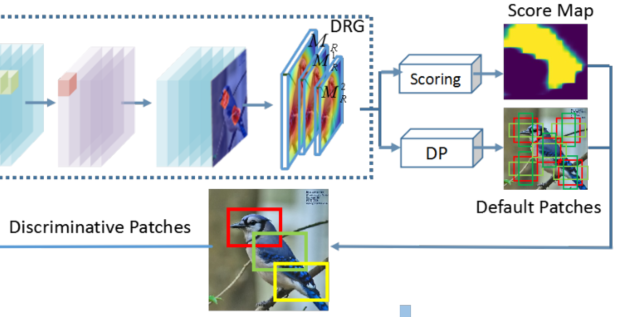
\includegraphics[width=0.35\textwidth]{docs/paperReading/CDL/dp.png}
        \end{figure}
        对残差模块生成的多尺度 $M_R^i(i=1,2,3)$ 计算 \textbf{discriminative probability maps} (Score Map) \footnote{$1\times 1$kernel+sigmoid} $S$,来表示判别区域对最终图像分类结果的影响。网络会选择top-N个个patch+区别的概率值$s_{ijk}$
        
        $p_{ijk}=tensor(t_x,t_y,t_w,t_h,s_{ijk})$
\end{multicols}
    
\end{frame}


\begin{frame}{Discriminative Feature Strengthening(DFS)}
    \begin{figure}
        \centering
        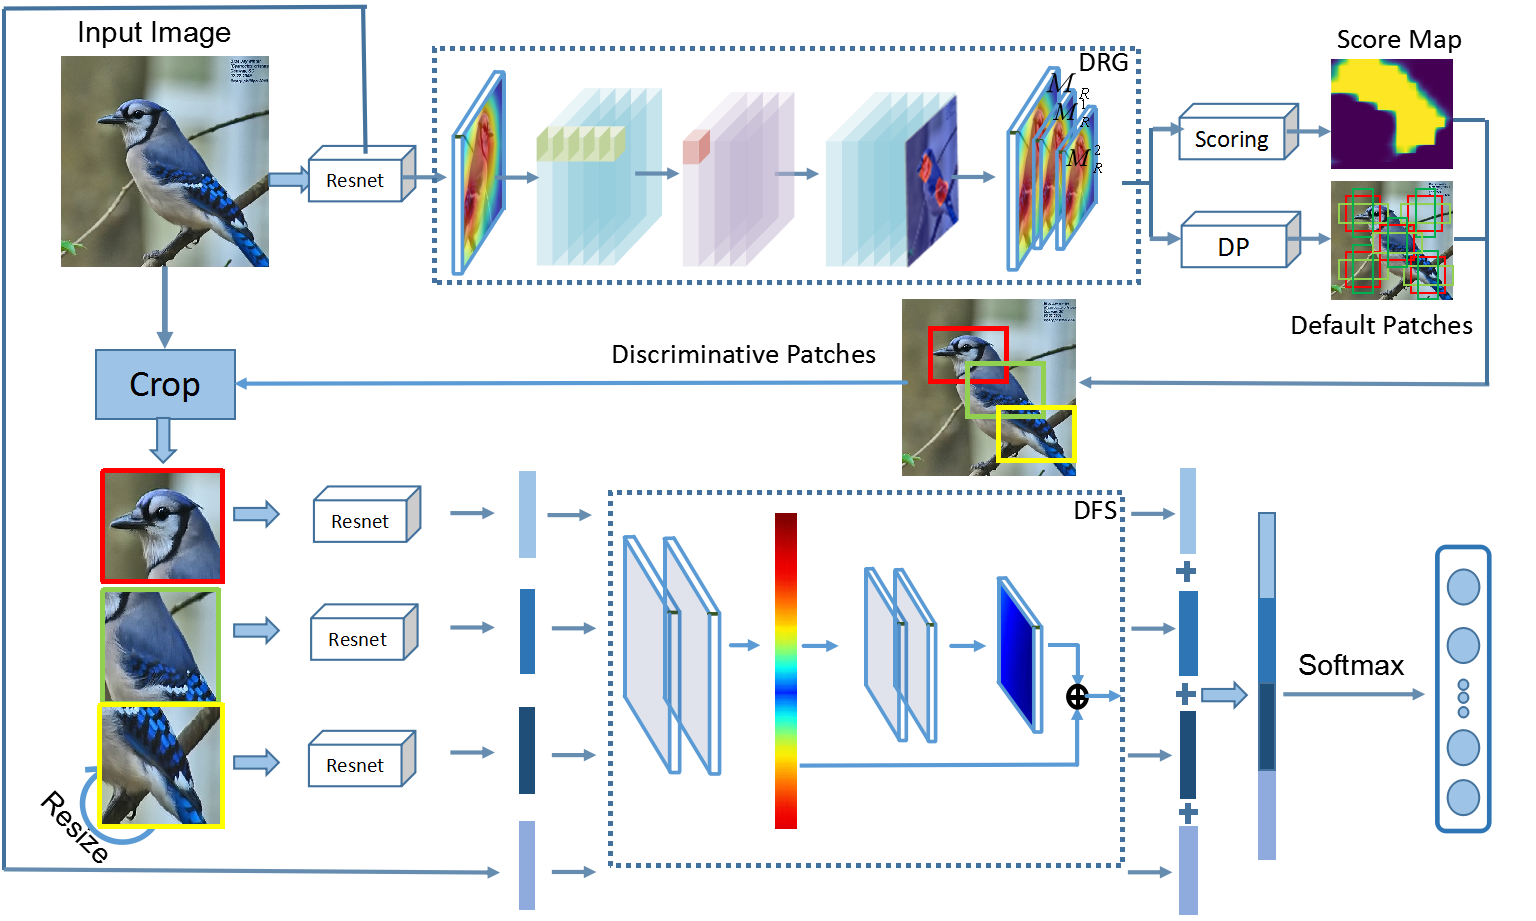
\includegraphics[width=0.6\textwidth]{docs/paperReading/CDL/framework.png}
        % \caption{\footnotesize framework of CDL}
    \end{figure}
    \textbf{DFS}(discriminative feature strengthening) 判别性特征增强子网络
\end{frame}
\begin{frame}{Discriminative Feature Strengthening(DFS)} 
    \begin{figure}
        \centering
        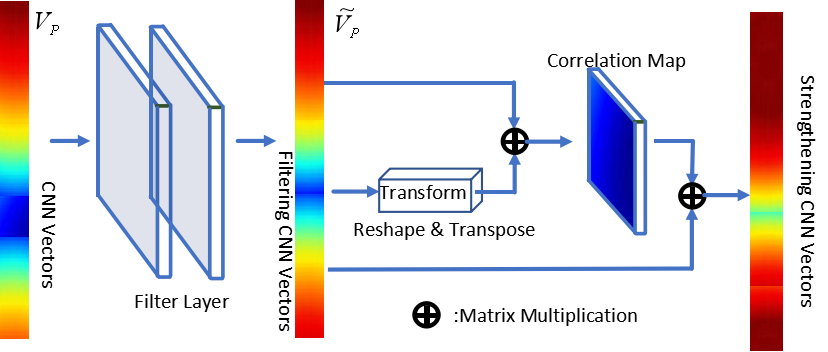
\includegraphics[width=0.5\textwidth]{docs/paperReading/CDL/dfs.png}
    \end{figure}
    \begin{scriptsize}
        \begin{enumerate}
            \item 过滤(filter layer)无用信息$\tilde{V_p}=ReLU(BN(W*V_p+b_p))$
            \item enhancement layer. $\tilde{S_E^{ij}}=softmax(S_E^{ij})=softmax(\tilde{V_pi}\cdot \tilde{V_pj}^T)$
            \item 经过增强的feature. $V=\tilde{V_p}\cdot \tilde{S_E}$
            \item 残差学习保证robustness. $\tilde{V}=\beta\cdot V+V_P$
        \end{enumerate}
    \end{scriptsize}
\end{frame}

\begin{frame}{Loss Function}
    \begin{scriptsize}
        \textbf{Multi-task loss} $\mathcal{L}$, 
        fine-grained classification loss$\mathcal{L}_{cls}$, 
        guided loss$\mathcal{L}_{gud}$, 
        correlation loss$\mathcal{L}_{rela}$, 
        rank loss $\mathcal{L}_{rank}$
        \begin{equation}
            \mathcal{L}=\mathcal{L}_{cls}
            +\lambda_1\cdot\mathcal{L}_{gud}
            +\lambda_2\cdot\mathcal{L}_{rela}
            +\lambda_3\cdot\mathcal{L}_{rank}
            \footnote{After many experiment verifications, set $\lambda_1=\lambda_2=\lambda_3=1$}
        \end{equation}
        
        \textbf{guided loss} $\mathcal{L}_{gud}$\footnote{$X$是原始图像,$C$是分类的置信度函数,选择的patch$P=\left\{P_1,P_2,...,P_N\right\}$和对应得分$S=\left\{S_1,S_2,...,S_N\right\}$}引导网络识别出更具判别性的区域。当所选区域的预测概率值低于整幅图像的预测概率值时,损失增加
        \begin{equation}
            \mathcal{L}_{gud}(X,P)=\sum_i^N max\left\{0,log{C(X)}-log{C(P_i)}\right\}
        \end{equation} 
        
        \textbf{correlation loss} $\mathcal{L}_{rela}$\footnote{$P_c$是所选择的特征的拼接}保证组合特征的预测概率大于单个特征的预测概率
        \begin{equation}
            \mathcal{L}_{rela}(P_c,P)=\sum_i^N max\left\{0,log{C(P_i)}-log{C(P_c)}\right\}
        \end{equation}
        
        \textbf{rank loss} $\mathcal{L}_{rank}$使得patch判别分数和最终分类概率一致,
        \begin{equation}
            \mathcal{L}_{rank}(S,P)=
            \sum_{log{C(P_i)}<log{C(P_j)}} (max\left\{0,(S_i-S_j)\right\})
        \end{equation}
    \end{scriptsize}
\end{frame}

\begin{frame}{Result:Quantitative Comparisons}
    \begin{wrapfigure}{l}{0.5\textwidth}    % 靠文字内容的左侧
        \centering
        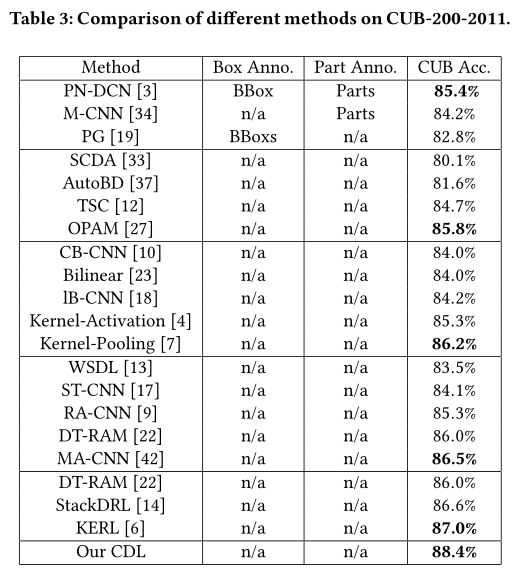
\includegraphics[width=0.35\textwidth]{docs/paperReading/CDL/comparison-1.png}        
    \end{wrapfigure}    
    \begin{scriptsize}
        \textbf{Accuracy Comparison.} \footnote{\textbf{Dataset}:Caltech-UCSD Bird-200-2011(CUB-200-2011)}        
        \begin{enumerate}
            \item supervised multi-stage methods
            \item weakly supervised multi-stage frameworks
            \item weakly supervised end-to-end feature encoding
            \item end-to-end localization-classification sub-networks
            \item other methods(reinforcement learning, knowledge representation)
            \item CDL.
        \end{enumerate}
        \textbf{Speed Comparison.}
        \begin{figure}
            \centering
            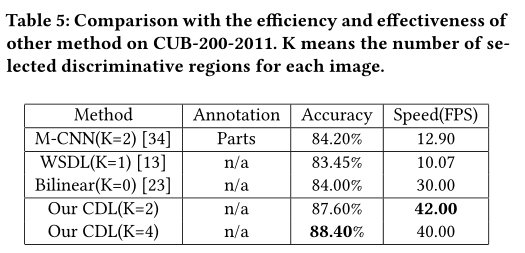
\includegraphics[width=0.35\textwidth]{docs/paperReading/CDL/comparison-2.png}
        \end{figure}
    \end{scriptsize}
\end{frame}


\begin{frame}{Result:Qualitative Analysis}
    \begin{multicols}{2}
        \begin{figure}
            \centering
            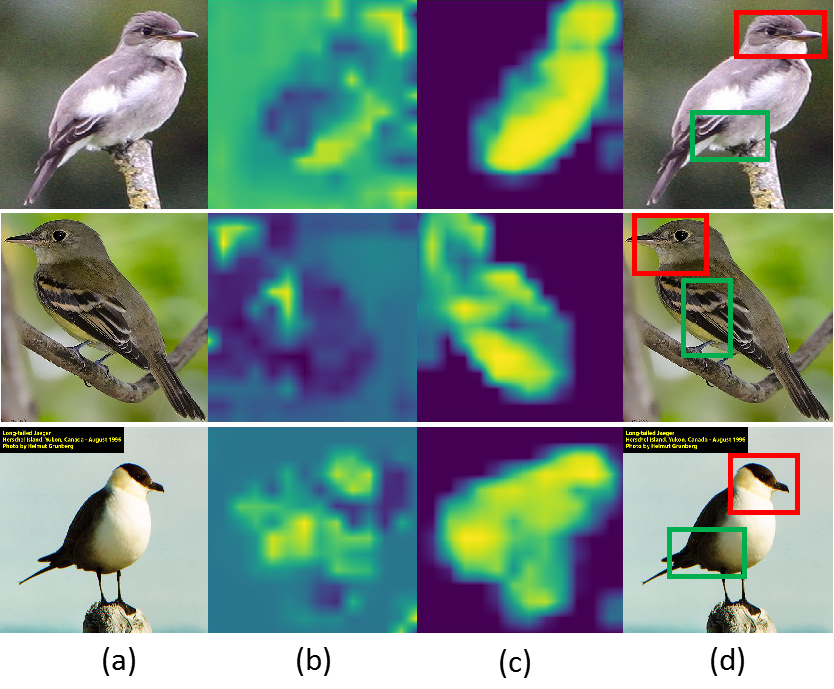
\includegraphics[width=0.32\textwidth]{docs/paperReading/CDL/result-2.png}
        \end{figure}
        \begin{scriptsize}
            判别性区域分组的可视化中间结果
            \begin{enumerate}
                \item \textbf{(a)}原始图像
                \item \textbf{(b)}相关性聚合的特征图$R^{ijk}$
                \item \textbf{(c)}残差特征图$M_R$
                \item \textbf{(d)}定位结果
            \end{enumerate}
        \end{scriptsize}  

        \begin{figure}
            \centering
            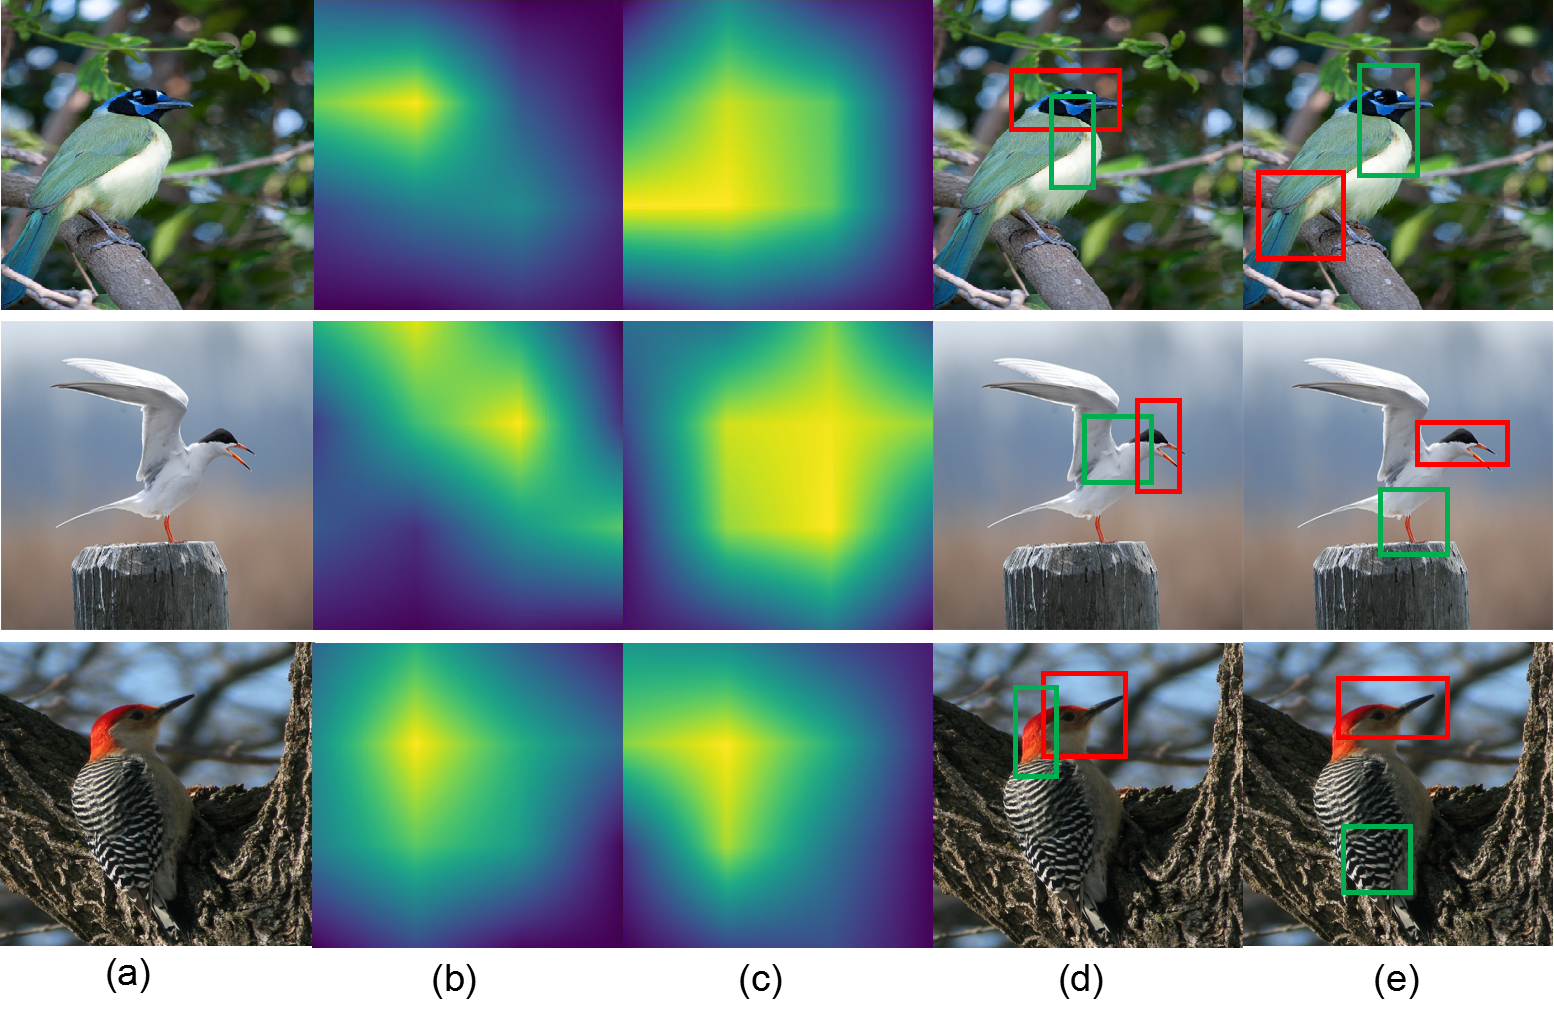
\includegraphics[width=0.4\textwidth]{docs/paperReading/CDL/result-3.png}
        \end{figure}
        \begin{scriptsize}
            区域间有无相关性的可视化定位结果
            \begin{enumerate}
                \item \textbf{(a)}原始图像
                \item \textbf{(b)(d)}无相关性判别的得分图、定位结果
                \item \textbf{(c)(e)}有相关性判别的得分图、定位结果
            \end{enumerate}
        \end{scriptsize}
    \end{multicols}
    
    
    
\end{frame}
% ----------------------------------------
% Non-local
% \section{Paper Reading: Non-Local}


\begin{frame}{Non-local Neural Networks (CVPR 2018)\cite{NonLocal2018}}
    \begin{itemize}
        \item \textbf{Title:}Non-local Neural Networks
        \item \textbf{Author:} Xiaolong Wang, Ross Girshick, Abhinav Gupta, Kaiming He\footnote{Carnegie Mellon University, Facebook AI Research}
        \item \textbf{Code:} https://github.com/facebookresearch/video-nonlocal-net
    \end{itemize}
\end{frame}


\begin{frame}{Non-local}
    \textbf{Non-local}
    \begin{equation}
        y_i=\frac{1}{C(x)}\sum_{\forall j}f(x_i,x_j)g(x_j)
    \end{equation}
    $C(x)$是归一化系数,$f(x_i,x_j)$用来计算输入信号在$x_j$位置与$x_i$的相似性/相关性,并且对$g(x_j)$进行加权,$g(x_j)$计算输入信号在$j$位置的特征值。
    \begin{itemize}
        \item \textbf{Gaussian.} $f(x_i,x_j)=e^{x_i^T x_j}$, $C(x)=\sum_{\forall j}f(x_i,x_j)$
        \item \textbf{Embedded Gaussian.} $f(x_i,x_j)=e^{\theta(x_i)^T \Phi(x_j)}$, $C(x)=\sum_{\forall j}f(x_i,x_j)$
        \item \textbf{Dot product.} $f(x_i,x_j)=\theta(x_i)^T \Phi(x_j)$, $C(x)=N$
        \item \textbf{Concatenation.} $f(x_i,x_j)=ReLU(w_f^T [\theta(x_i),\Phi(x_j)])$, $C(x)=N$
    \end{itemize}
\end{frame}

\begin{frame}{Non-local}
    \begin{multicols}{2}
        \begin{figure}
            \centering
            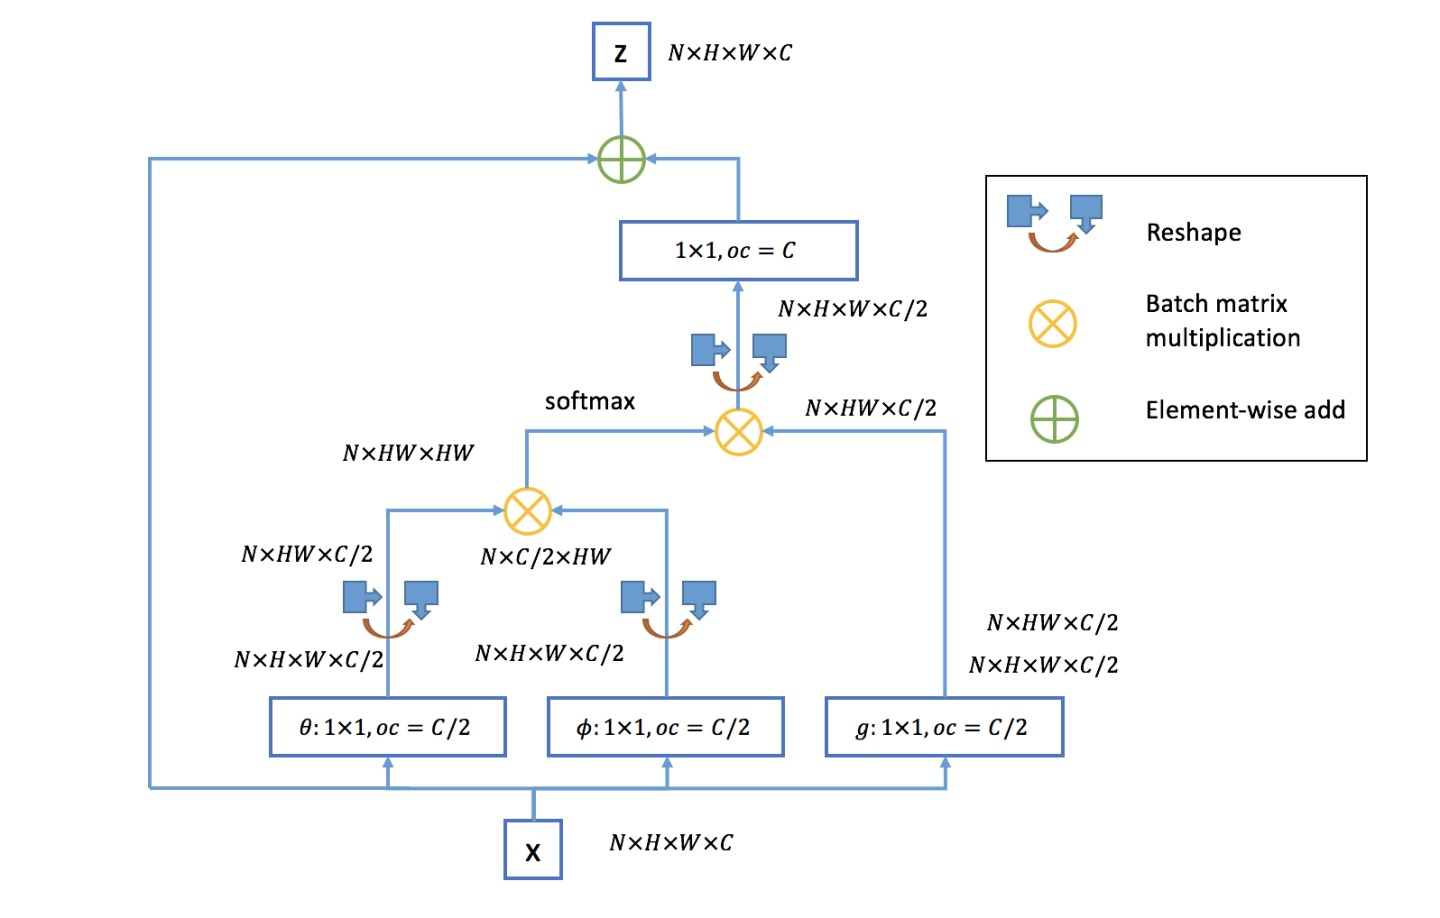
\includegraphics[width=0.6\textwidth]{docs/paperReading/Non-local/non-local.jpg}
        \end{figure}
        

        \textbf{Non-local Block}
        \begin{equation}
            z_i=W_z y_i+x_i
        \end{equation}
        \hspace*{\fill}
        \hspace*{\fill}
        \hspace*{\fill}
        \begin{equation}
            y_i=Softmax(\theta(x_i)^T \Phi(x_j))g(x_j)
        \end{equation}
        $\theta(x_i)$表示局部,$\Phi(x_i)$是

    \end{multicols}
\end{frame}

\begin{frame}{Experiment in Kinetics Dataset}    
    \begin{multicols}{2}       
        \begin{figure}
            \centering
            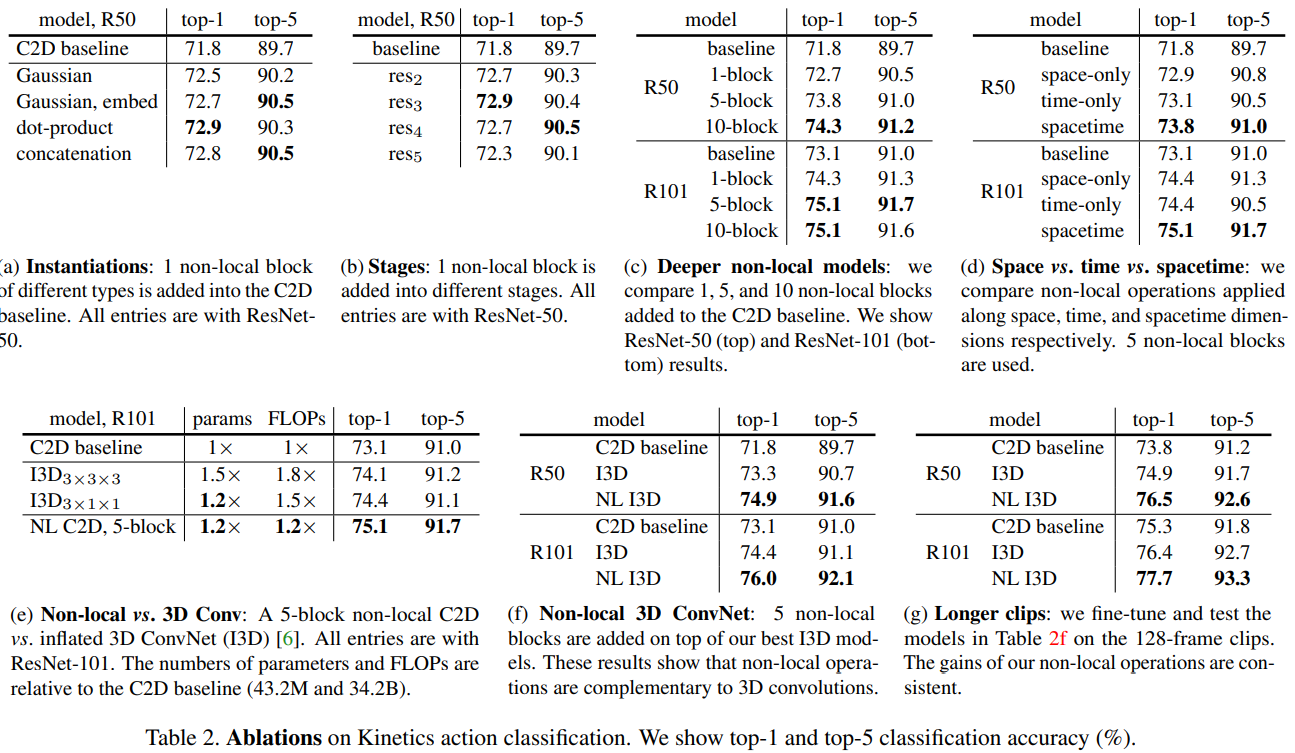
\includegraphics[width=0.54\textwidth]{docs/paperReading/Non-local/exp.png}
        \end{figure}

        \begin{scriptsize}
            Kinetics Dataset: 行为识别 benchmark
            \begin{itemize}
                \item (a) 四种相似度计算模型$f$对比
                \item (b) non-local加在ResNet-50不同的stage下。在stage3,4添加提升acc较大
                \item (c) 在ResNet-50和ResNet-101中添加不同数量的non-local block。添加数量越多,效果越好
                \item (d) 在
                \item (e) 与3D Conv在参数量、计算量、acc进行对比
                \item (f) 在3D Conv加入non-local模块
            \end{itemize}
        \end{scriptsize}
    \end{multicols}
\end{frame}

\begin{frame}{Experiment}    
    \begin{figure}
        \centering
        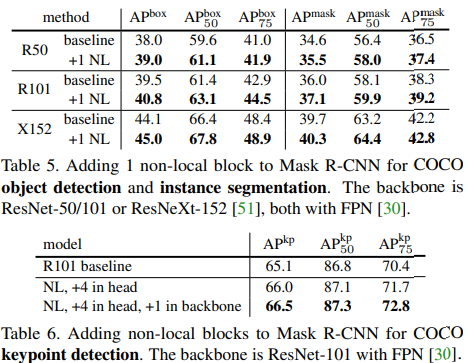
\includegraphics[width=0.5\textwidth]{docs/paperReading/Non-local/assignment.png}
    \end{figure}

    \begin{scriptsize}
        基于COCO数据集,Non-local应用在object detection, instance segmentation, keypoint detection等任务上
    \end{scriptsize}
\end{frame}


\begin{frame}{Experiment(*)}
    \begin{multicols}{2}
        \begin{tiny}
            将Non-local block添加到网络中,分别是:

            \textbf{ResNet-50}

            \textbf{ResNet-50 Non-local layer-1}: 在 $layer1$ 后添加 $1$ 个Non-Local Block

            \textbf{ResNet-50 Non-local layer-2}: 在 $layer2$ 后添加 $1$ 个Non-Local Block

            \textbf{ResNet-50 Non-local layer-3}: 在 $layer3$ 后添加 $1$ 个Non-Local Block

            \textbf{ResNet-50 Non-local layer-4}: 在 $layer4$ 后添加 $1$ 个Non-Local Block

            \textbf{ResNet-50 Non-local 5-block}: 在 $layer3$ 后添加 $3$ 个、在 $layer4$ 后添加 $2$ 个,共5个Non-Local Block

            \textbf{ResNet-50 Non-local 10-block}: 在 $layer3$ 后添加 $5$ 个、在 $layer4$ 后添加 $5$ 个,共10个Non-Local Block
        \end{tiny}

        \begin{figure}
            \centering
            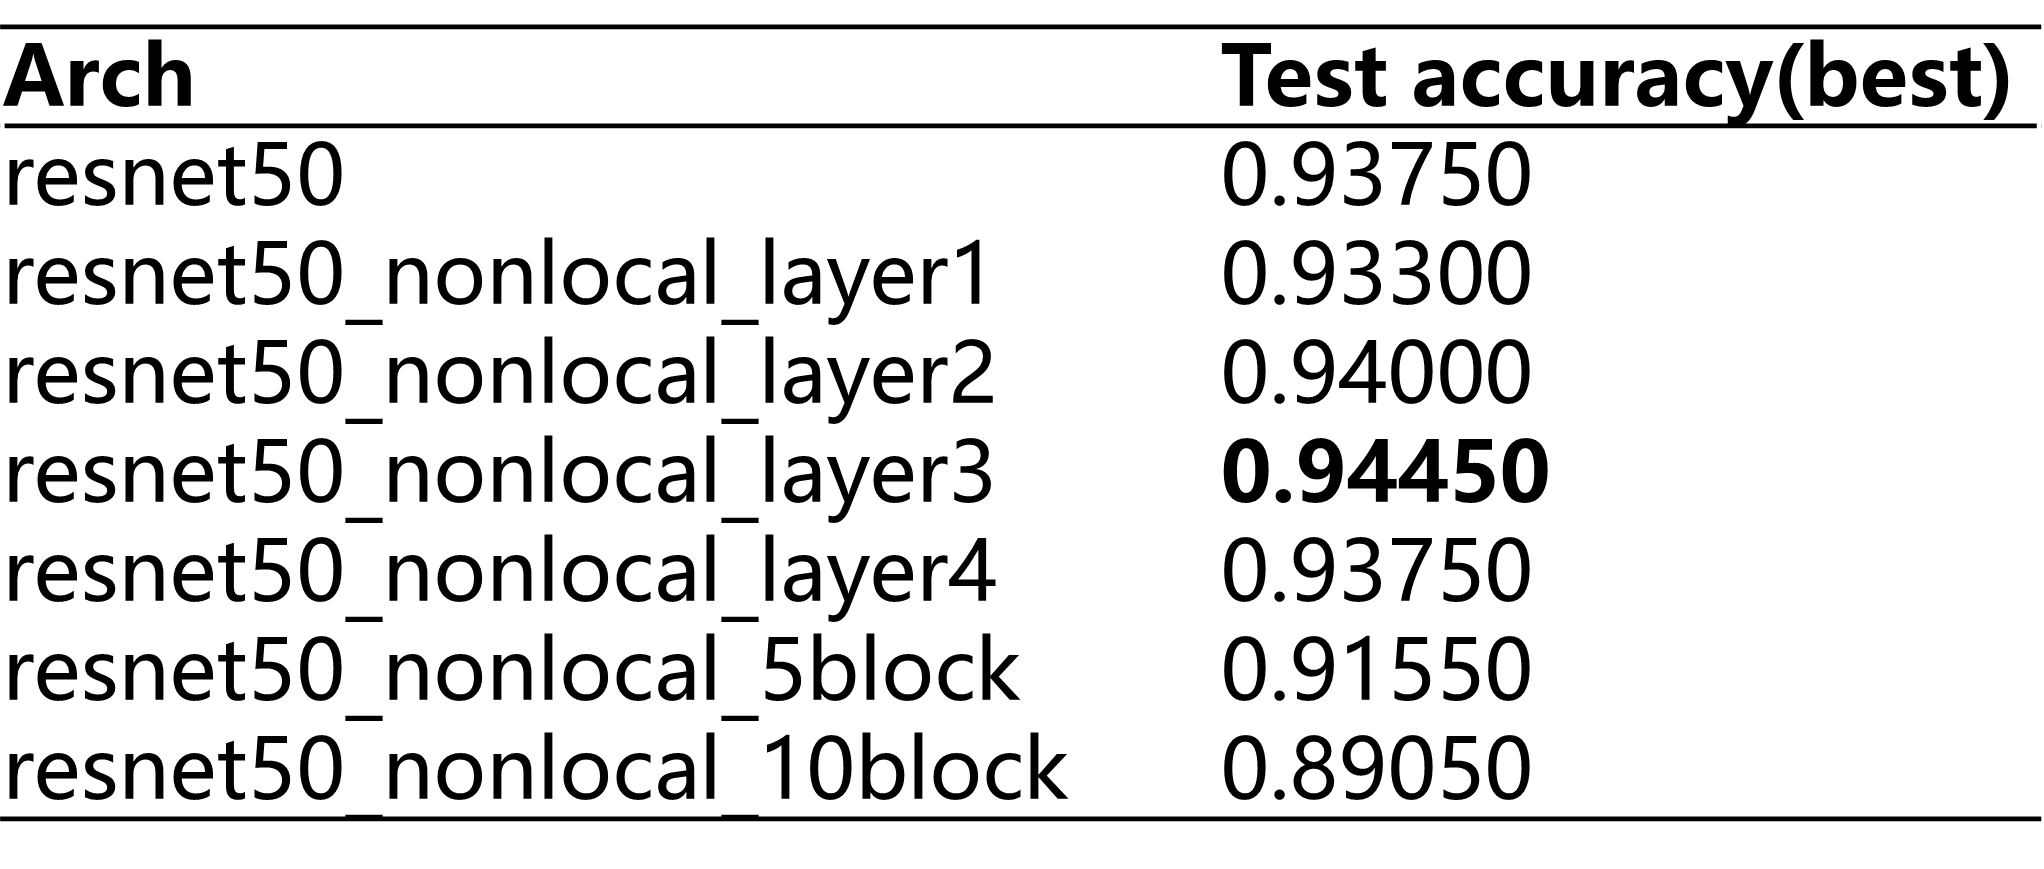
\includegraphics[width=0.37\textwidth]{docs/paperReading/Non-local/table.png}
        \end{figure}
        \begin{figure}
            \centering
            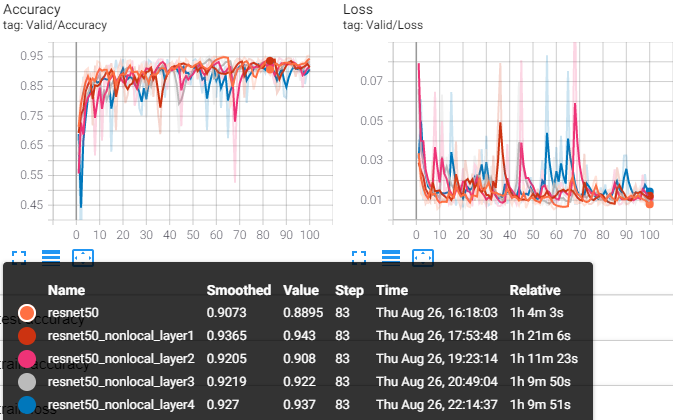
\includegraphics[width=0.37\textwidth]{docs/paperReading/Non-local/testacc-1.png}
            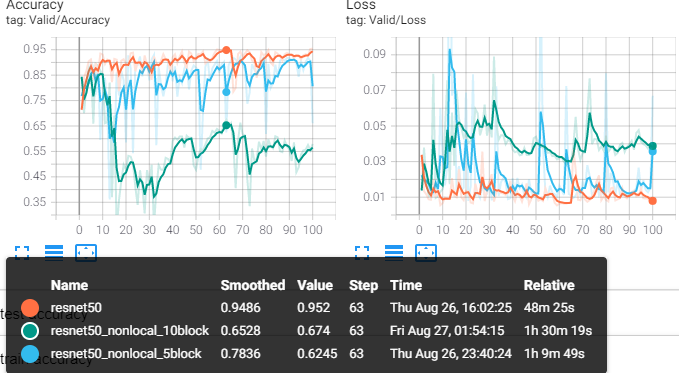
\includegraphics[width=0.37\textwidth]{docs/paperReading/Non-local/testacc-2.png}
        \end{figure}
    \end{multicols}
\end{frame}

\begin{frame}{Experiment(*)}
    \begin{multicols}{2}
    \begin{figure}
        \centering
        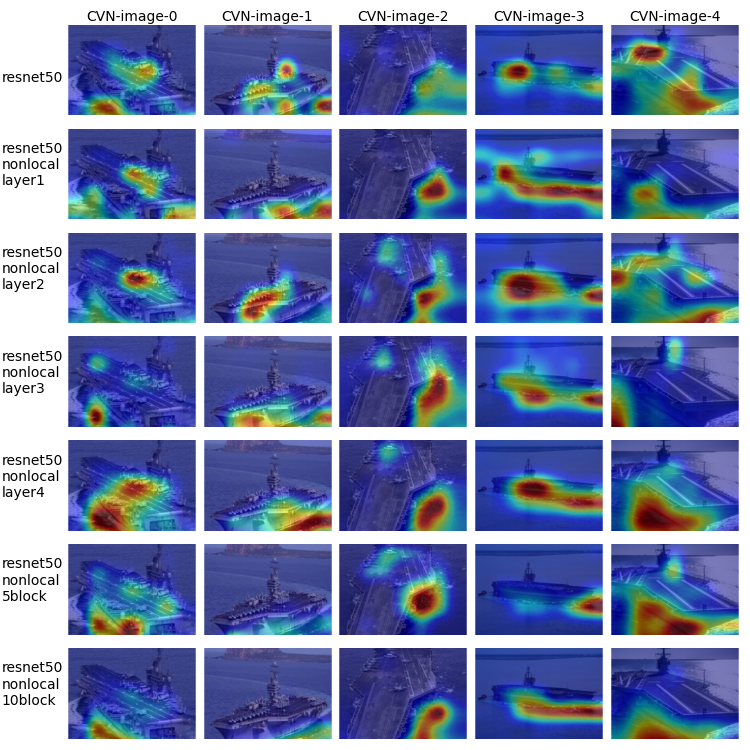
\includegraphics[width=0.45\textwidth]{docs/paperReading/Non-local/exp/CVN.png}
    \end{figure}

    \begin{scriptsize}
        图中从上至下,分别是:

        \begin{tiny}
            \textbf{ResNet-50}

            \textbf{ResNet-50 Non-local layer-1}: 在 $layer1$ 后添加 $1$ 个Non-Local Block

            \textbf{ResNet-50 Non-local layer-2}: 在 $layer2$ 后添加 $1$ 个Non-Local Block

            \textbf{ResNet-50 Non-local layer-3}: 在 $layer3$ 后添加 $1$ 个Non-Local Block
            
            \textbf{ResNet-50 Non-local layer-4}: 在 $layer4$ 后添加 $1$ 个Non-Local Block
            
            \textbf{ResNet-50 Non-local 5-block}: 在 $layer3$ 后添加 $3$ 个、在 $layer4$ 后添加 $2$ 个,共5个Non-Local Block
            
            \textbf{ResNet-50 Non-local 10-block}: 在 $layer3$ 后添加 $5$ 个、在 $layer4$ 后添加 $5$ 个,共10个Non-Local Block
        \end{tiny}

        类别: CVN 
    \end{scriptsize}
\end{multicols}
\end{frame}

\begin{frame}{Experiment(*)}
    \begin{multicols}{2}
        \begin{figure}
            \centering
            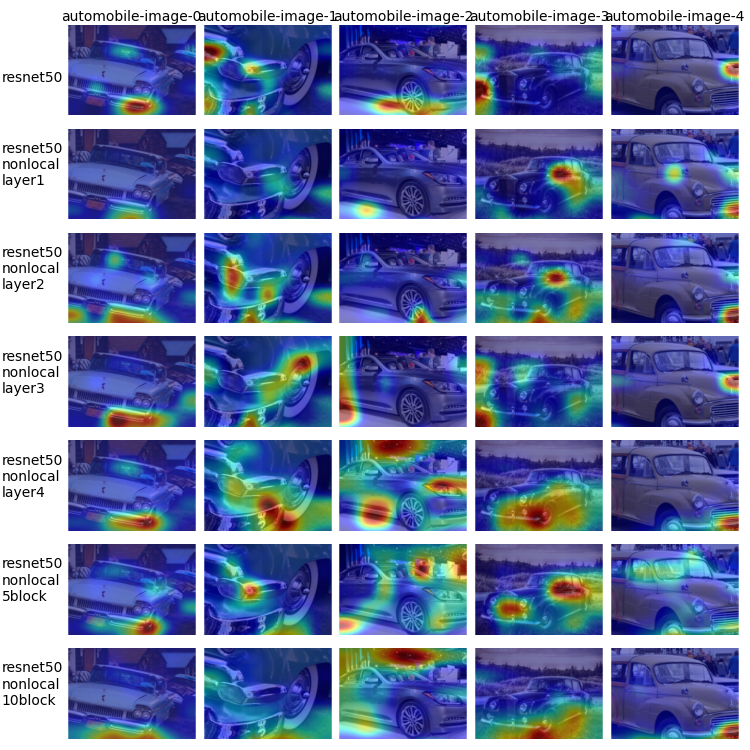
\includegraphics[width=0.45\textwidth]{docs/paperReading/Non-local/exp/automobile.png}
        \end{figure}

        \begin{scriptsize}
            图中从上至下,分别是:

            \begin{tiny}
                \textbf{ResNet-50}

                \textbf{ResNet-50 Non-local layer-1}: 在 $layer1$ 后添加 $1$ 个Non-Local Block

                \textbf{ResNet-50 Non-local layer-2}: 在 $layer2$ 后添加 $1$ 个Non-Local Block

                \textbf{ResNet-50 Non-local layer-3}: 在 $layer3$ 后添加 $1$ 个Non-Local Block
                
                \textbf{ResNet-50 Non-local layer-4}: 在 $layer4$ 后添加 $1$ 个Non-Local Block
                
                \textbf{ResNet-50 Non-local 5-block}: 在 $layer3$ 后添加 $3$ 个、在 $layer4$ 后添加 $2$ 个,共5个Non-Local Block
                
                \textbf{ResNet-50 Non-local 10-block}: 在 $layer3$ 后添加 $5$ 个、在 $layer4$ 后添加 $5$ 个,共10个Non-Local Block
            \end{tiny}

            类别: automobile 
        \end{scriptsize}
    \end{multicols}
\end{frame}
% cargo_ship
\begin{frame}{Experiment(*)}
    \begin{multicols}{2}
        \begin{figure}
            \centering
            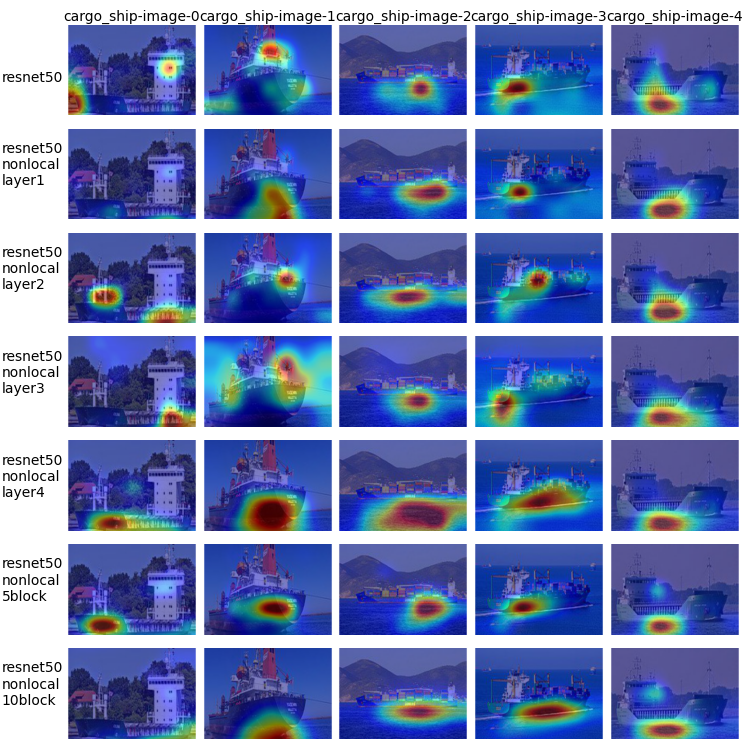
\includegraphics[width=0.45\textwidth]{docs/paperReading/Non-local/exp/cargo_ship.png}
        \end{figure}

        \begin{scriptsize}
            图中从上至下,分别是:

            \begin{tiny}
                \textbf{ResNet-50}

                \textbf{ResNet-50 Non-local layer-1}: 在 $layer1$ 后添加 $1$ 个Non-Local Block

                \textbf{ResNet-50 Non-local layer-2}: 在 $layer2$ 后添加 $1$ 个Non-Local Block

                \textbf{ResNet-50 Non-local layer-3}: 在 $layer3$ 后添加 $1$ 个Non-Local Block
                
                \textbf{ResNet-50 Non-local layer-4}: 在 $layer4$ 后添加 $1$ 个Non-Local Block
                
                \textbf{ResNet-50 Non-local 5-block}: 在 $layer3$ 后添加 $3$ 个、在 $layer4$ 后添加 $2$ 个,共5个Non-Local Block
                
                \textbf{ResNet-50 Non-local 10-block}: 在 $layer3$ 后添加 $5$ 个、在 $layer4$ 后添加 $5$ 个,共10个Non-Local Block
            \end{tiny}

            类别: cargo ship 
        \end{scriptsize}
    \end{multicols}
\end{frame}
% \section{图像去噪算法: Non-Local Mean 非局部均值滤波}



\begin{frame}{Non-local Means 非局部均值滤波}
    原始图像$v$的每个像素点$v(x)$经过滤波之后可以得到对应图像上的点$\tilde{u}(x)$
    \begin{equation}
        \tilde{u}(x)=\sum_{y\in \Omega_x} w(x,y)v(y)
        \label{nl-mean}
    \end{equation}    
    公式\ref{nl-mean}中,$w(x,y)$是一个权重,表示在原始图像$v$中,像素$x$、$y$之间的相似性。$\Omega_x$是像素$x$的邻域。同时权重需要满足公式\ref{nl-mean-weight_condition}的条件
    \begin{equation}
        w(x,y)>0\quad and\quad \sum_{y\in \Omega_x} w(x,y)=1,\forall x\in \Omega,y\in \Omega_x
        \label{nl-mean-weight_condition}
    \end{equation}

    对于每一个像素,其去噪后的结果等于其邻域中像素$y$的加权和,权重则是像素$x$、$y$之间的相似性。该邻域称为“搜索邻域”,其范围越大,可以找到相似的概率也就越大大,但是计算量也会增大。
\end{frame}

\begin{frame}{Non-local Means 非局部均值滤波}
    用欧氏距离来衡量两个像素之间的相似性
    \begin{equation}
        w(x,y)=\frac{1}{n(x)} \exp(\frac{||V(x)-V(y)||_{2,a}^2}{h^2})
    \end{equation}
    $n(x)$是归一化因子,是所有权重和,使得满足公式\ref{nl-mean-weight_condition}中权重和为1的条件。

    $V(x)$和$V(y)$分别是像素$x$和$y$的块(Patch)邻域,小于搜索邻域。
    $||V(x)-V(y)||_{2,a}^2$是两个邻域的的\textbf{高斯加权欧氏距离}\footnote{求欧式距离的时候,距离块邻域的中心越近的权重越大,越远则越小,权重服从高斯分布,因此需要在距离上乘以一个高斯权重。},高斯权重为:    
    \begin{equation}
        G(x,y)=\frac{1}{2\pi a^2}\exp(-\frac{(x^2+y^2)}{2a^2})
    \end{equation}
\end{frame}


\begin{frame}{Non-local filter}
    \begin{figure}
        \centering
        \includegraphics[width=0.65\textwidth]{docs/paperReading/Non-local/non-local-means.png}
    \end{figure}
\end{frame}


% ----------------------------------------
% DANet
% \section{Paper Reading: DANet (TODO)}


\begin{frame}{Dual Attention Network for Scene Segmentation}
    \begin{itemize}
        \item \textbf{Title:} Dual Attention Network for Scene Segmentation
        \item \textbf{Author:} Jun Fu, Jing Liu, Haijie Tian, Yong Li, Yongjun Bao, Zhiwei Fang, Hanqing Lu
        \item \textbf{Comments:} Accepted by CVPR2019
        % \item \textbf{Contribution:} \textbf{Propose} an end-to-end Correlation-guided Discriminative Learning (CDL) model to fully mine and exploit the discriminative potentials of correlations for WFGIC globally and locally. 
        % \footnote{提出了一个端到端相关性引导判别学习(CDL)模型,以充分挖掘和利用相关性在全局和局部的鉴别潜力。}
        % \item 开源代码:无
        
        \item \textbf{arxiv:}https://arxiv.org/pdf/1809.02983.pdf
    \end{itemize}
\end{frame}


\begin{frame}{Non-local}
    \textbf{Non-local}
    \begin{equation}
        y_i=\frac{1}{C(x)}\sum_{\forall j}f(x_i,x_j)g(x_j)
    \end{equation}
    $C(x)$是归一化系数,$f(x_i,x_j)$用来计算输入信号在$x_j$位置与$x_i$的相似性/相关性,并且对$g(x_j)$进行加权,$g(x_j)$计算输入信号在$j$位置的特征值。
    \begin{itemize}
        \item \textbf{Gaussian.} $f(x_i,x_j)=e^{x_i^T x_j}$, $C(x)=\sum_{\forall j}f(x_i,x_j)$
        \item \textbf{Embedded Gaussian.} $f(x_i,x_j)=e^{\theta(x_i)^T \Phi(x_j)}$, $C(x)=\sum_{\forall j}f(x_i,x_j)$
        \item \textbf{Dot product.} $f(x_i,x_j)=\theta(x_i)^T \Phi(x_j)$, $C(x)=N$
        \item \textbf{Concatenation.} $f(x_i,x_j)=ReLU(w_f^T [\theta(x_i),\Phi(x_j)])$, $C(x)=N$
    \end{itemize}
\end{frame}

\begin{frame}{DANet}
    \begin{figure}
        \centering
        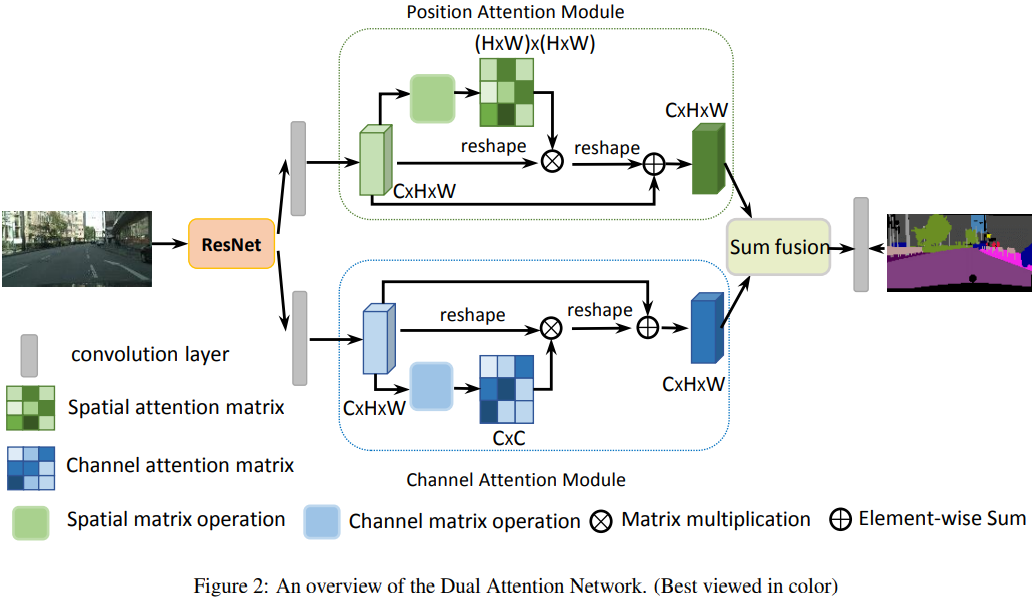
\includegraphics[width=0.8\textwidth]{docs/paperReading/danet/danet.png}
    \end{figure}
\end{frame}

\begin{frame}{DANet:PAM and CAM}
    \begin{figure}
        \centering
        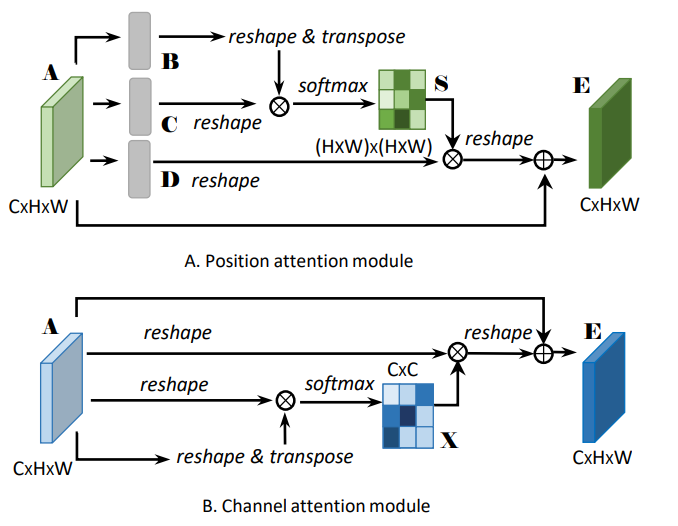
\includegraphics[width=0.45\textwidth]{docs/paperReading/danet/pam_cam.png}
    \end{figure}

    \begin{itemize}
        \item \textbf{PAM} Position attention module
        \item \textbf{CAM} Channel attention module
    \end{itemize}
\end{frame}


% \begin{frame}{experiment}
%     \begin{multicols}{2}
%         \begin{figure}
%             \centering
%             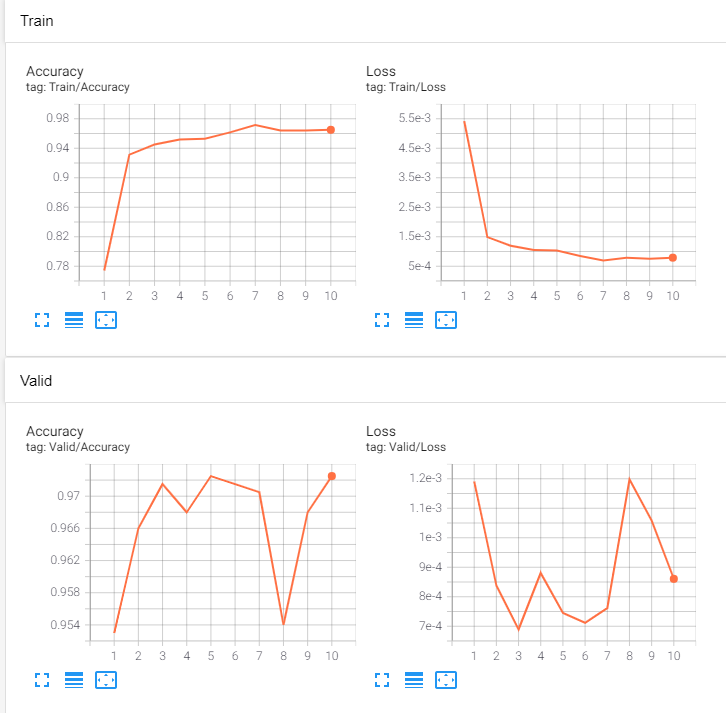
\includegraphics[width=0.4\textwidth]{docs/paperReading/danet/lr_0001.png}
%             \caption{lr=0.0001}
%         \end{figure} 
%         \begin{figure}
%             \centering
%             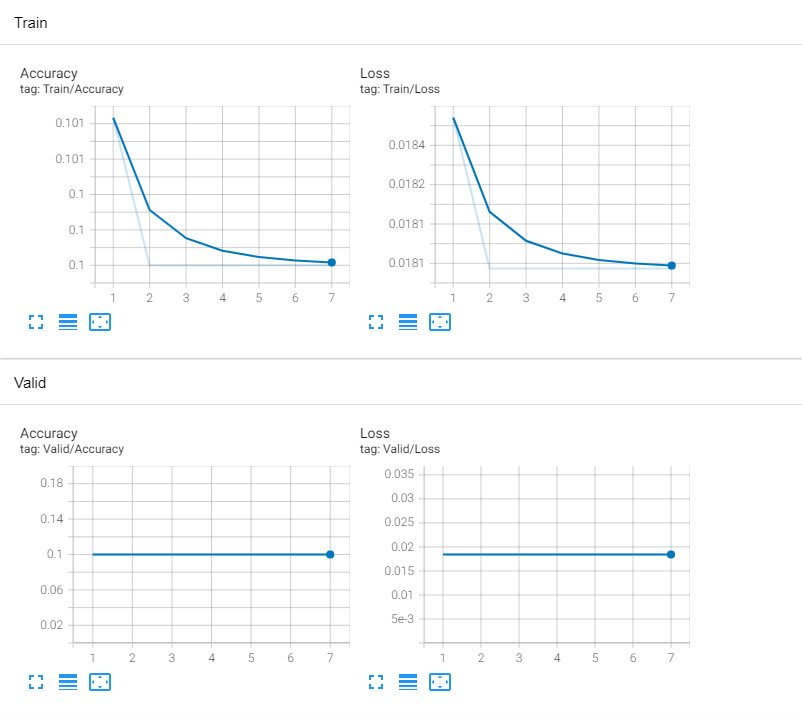
\includegraphics[width=0.4\textwidth]{docs/paperReading/danet/lr_001.png}
%             \caption{lr=0.001}
%         \end{figure} 
%     \end{multicols}
% \end{frame}

% ----------------------------------------
% SENet
% \section{Paper Reading: SENet (TODO)}


\begin{frame}{Squeeze-and-Excitation Networks}
    \begin{itemize}
        \item \textbf{Author:} Jie Hu, Li Shen, Gang Sun
        \item \textbf{Comments:} Accepted by CVPR2019
    \end{itemize}
\end{frame}

% ----------------------------------------
% CBAM
% \section{Paper Reading: CBAM (TODO)}

% ----------------------------------------
% CW attack
% \section{CW attack}


\begin{frame}{CW attack}
    \begin{itemize}
        \item \textbf{Title:}Towards Evaluating the Robustness of Neural Networks
        \item \textbf{Author:} Nicholas Carlini, David Wagner\footnote{University of California, Berkeley}
        % \item \textbf{Contribution}
    \end{itemize}
\end{frame}

\begin{frame}{生成对抗样本的思路}
    CW攻击是一种基于优化的攻击方式,其攻击思路主要有
    \begin{itemize}
        \item 添加的扰动尽量小,$x+\delta \in [0,1]^n$
        \item 对抗样本和干净样本的距离越小越好,即$\text{minimize}\quad D(x,x+\delta)$
        \item 对抗样本应该使得模型分类错误$C(x+\delta)=t$,且分类错误的概率越高越好
    \end{itemize}

    对抗样本的公式:原始样本$x$和生成的对抗样本$x+\delta$之间的距离为$D(x,x+\delta)$,使得模型$C$在输入对抗样本$x+\delta$的情况下,产生错误的分类预测结果$t$。
    \begin{equation}
        \begin{aligned}
            \text{minimize}\quad    & D(x,x+\delta) \\
            \text{such that}\quad   & C(x+\delta)=t \\
                                    & x+\delta \in [0,1]^n
        \end{aligned}
        \label{L-BFGS}
    \end{equation}    
\end{frame}

\begin{frame}{构建对抗样本}
    但是由于$C$是高度非线性的,公式\ref{L-BFGS}很难求解,因此文中定义一个目标函数$f$,使得$C(x+\delta)=t$当且仅当$f(x+\delta)\leq 0$,上面的公式就可以变成
    \begin{equation}
        \begin{aligned}
            \text{minimize}\quad    & D(x,x+\delta)+c\cdot f(x+\delta) \\
            \text{such that}\quad   & C(x+\delta)=t \\
                                    & x+\delta \in [0,1]^n
        \end{aligned}
    \end{equation}
    $c$是一个超参数,并且$c>0$。
\end{frame}


\begin{frame}{构建对抗样本}
    \begin{multicols}{2}
        \begin{figure}
            \centering
            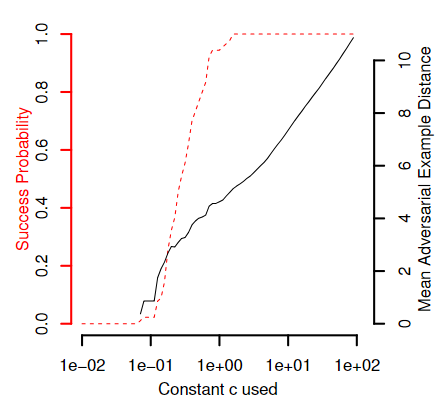
\includegraphics[width=0.4\textwidth]{docs/paperReading/CW_attack/const-c.png}
        \end{figure}
        实验发现,随着参数$c$的增大,攻击成功率(左侧红色虚线)和对抗样本平均距离(也就是对抗扰动,右侧黑色实线)也都会增大。在$c=0.1$附近的取值能够使得攻击成功率较小的情况下,扰动也较小
    \end{multicols}
\end{frame}


\begin{frame}{构建对抗样本}    
    需要对扰动$\delta_i$添加一个约束(论文中称为 Box constraints),$0\leq x_i+\delta_i\leq 1$

    引入参数$\omega_i$,假定
    \begin{equation}
        -1\leq \tanh(\omega_i)\leq 1
    \end{equation}
    那么
    \begin{equation}
        0\leq \frac{1}{2}(\tanh(\omega_i)+1)\leq 1
    \end{equation}
    可以得到CW方法中对$\delta_i$的约束
    \begin{equation}
        x_i+\delta_i=\frac{1}{2}(\tanh(\omega_i)+1)
    \end{equation}
    公式就可以改写成
    \begin{equation}
        \begin{aligned}
            \text{minimize}\quad    & D(x,x+\delta)+c\cdot f(\frac{1}{2}(\tanh(\omega_i)+1)) \\
            \text{such that}\quad   & C(x+\delta)=t \\
                                    & x+\delta \in [0,1]^n
        \end{aligned}
    \end{equation}

\end{frame}


\begin{frame}{构建对抗样本}
    对于公式中的$f$
    \begin{equation}
        \begin{aligned}
            f_1(x') & = -loss_{F,t}(x')+1 \\
            f_2(x') & = [\mathop{\max}\limits_{i\neq t}(F(x')_i)-F(x')_t]^+ \\
            f_3(x') & = \text{softplus}[\mathop{\max}\limits_{i\neq t}(F(x')_i)-F(x')_t]-\log(2) \\
            f_4(x') & = (0.5-F(x')_t)^+ \\
            f_5(x') & = -\log(2F(x')_t-2)^+ \\
            f_6(x') & = [\mathop{\max}\limits_{i\neq t}(Z(x')_i)-Z(x')_t]^+ \\
            f_7(x') & = \text{softplus}[\mathop{\max}\limits_{i\neq t}(Z(x')_i)-Z(x')_t]-\log(2)
        \end{aligned}
    \end{equation}
    其中$(e)^+=max(e,0)$,$\text{softplus}(x)=\log(1+e^x)$,$\text{loss}_{F,s}(x)$是$x$的交叉熵损失
\end{frame}


\begin{frame}{构建对抗样本}
    \begin{scriptsize}
        距离$D(x,x+\delta)$的计算可以选择$L_1,L_2,L_\infty$三种
        \begin{itemize}
            \item $L_2$ 攻击
        \end{itemize}
        \begin{equation}
            \begin{aligned}
                \text{minimize}\quad ||\frac{1}{2}(\tanh(\omega)+1)-x||_2^2+c\cdot f(\frac{1}{2}(\tanh(\omega_i)+1)) \\
                f(x')=\max(\max\left\{Z(x')_i:i\neq t\right\}-Z(x')_t,-\kappa),\quad set \kappa=0
            \end{aligned}
        \end{equation}


        \begin{itemize}
            \item $L_0$ 攻击
        \end{itemize}
        $L_0$距离度量是不可微的,因此不适合标准梯度下降。作者使用迭代算法,在每次迭代中,识别对输出结果没有太大影响的像素,并且固定其数值不做修改。

        \begin{itemize}
            \item $L_\infty$ 攻击
        \end{itemize}
        $L_\infty$距离度量效果并不好,作者使用了迭代攻击来解决这个问题
        \begin{equation}
            \text{minimize}\quad \sum[(\delta_i-\tau)^+]+c\cdot f(\frac{1}{2}(\tanh(\omega_i)+1))
        \end{equation}
        $(\delta_i-\tau)^+=\max(\delta_i-\tau,0)$,惩罚任何超过$\tau$的扰动$\delta_i$,$0.9\leq \tau\leq 1$,\(\tau\)从1开始减小,小于0.9时停止
    \end{scriptsize}
\end{frame}

\begin{frame}{实验}
    三种范数下的CW攻击(MNIST数据集)结果
    \begin{figure}
        \centering
        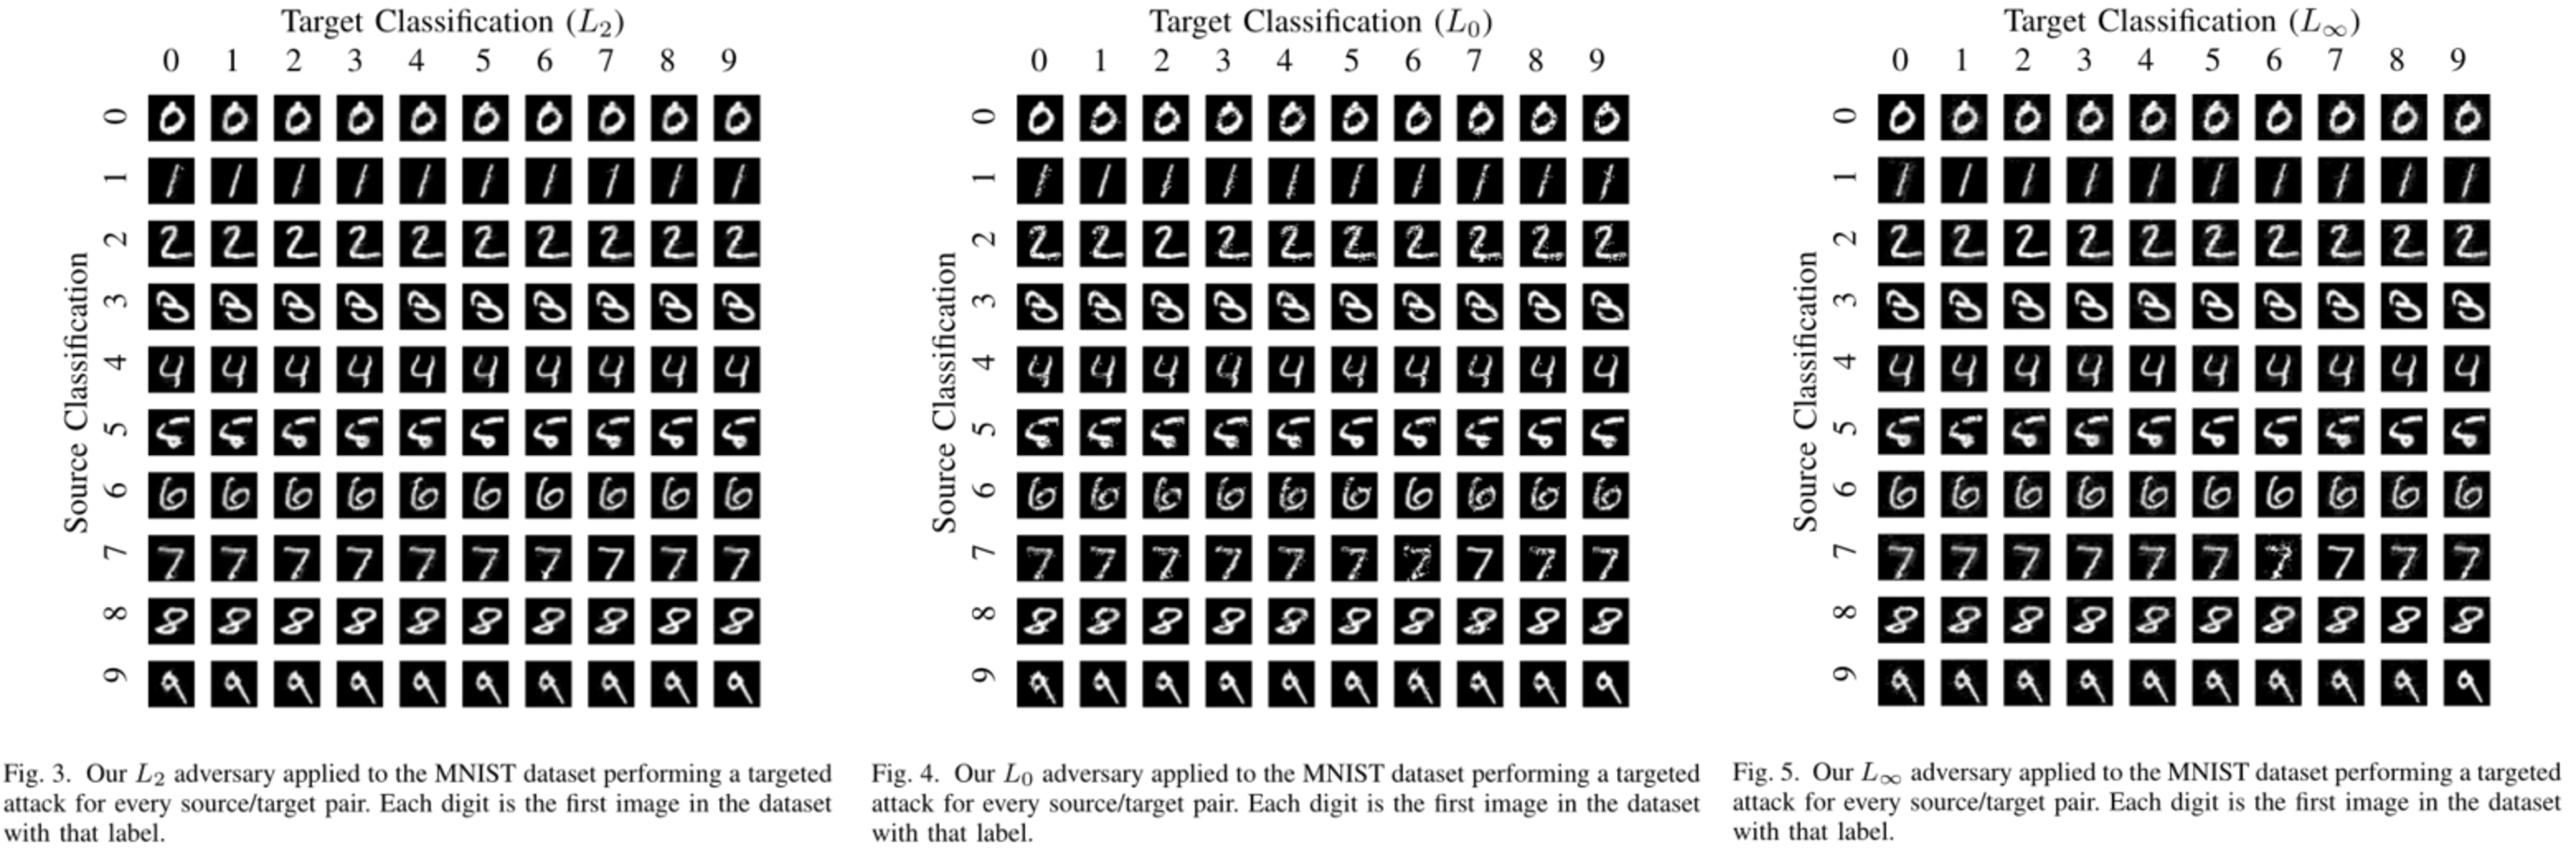
\includegraphics[width=1.0\textwidth]{docs/paperReading/CW_attack/attack-sample.png}
    \end{figure}
\end{frame}


\begin{frame}{实验}
    CW的攻击扰动都很小
    \begin{figure}
        \centering
        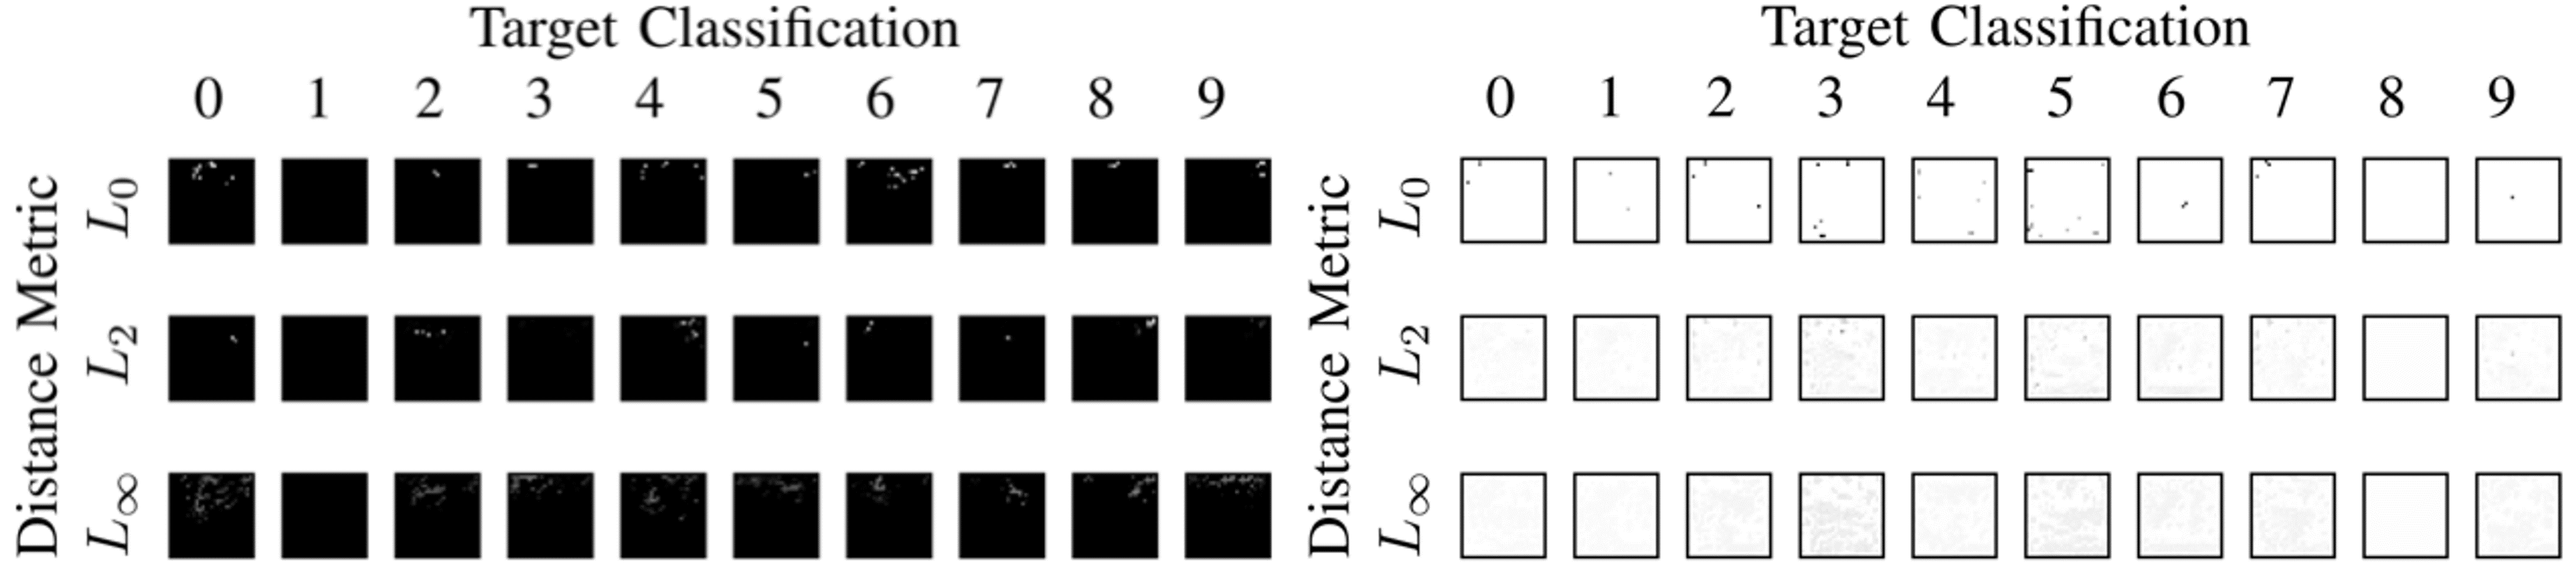
\includegraphics[width=1.0\textwidth]{docs/paperReading/CW_attack/per.png}
    \end{figure}
\end{frame}

\begin{frame}{实验}
    作者对ImageNet进行攻击,攻击扰动也很小
    \begin{figure}
        \centering
        \includegraphics[width=0.9\textwidth]{docs/paperReading/CW_attack/imagenet.png}
    \end{figure}
\end{frame}

\begin{frame}{实验}
    $L_2$的攻击扰动小,但是攻击的速度很慢
    \begin{figure}
        \centering
        \includegraphics[width=1.05\textwidth]{docs/paperReading/CW_attack/cw-exp.png}
    \end{figure}    
\end{frame}
% ----------------------------------------
% DeepFool attack
% \section{DeepFool attack}

\begin{frame}{DeepFool attack}
    \begin{itemize}
        \item \textbf{Title:} DeepFool: a simple and accurate method to fool deep neural networks (CVPR 2016)
        \item \textbf{Author:} Seyed-Mohsen Moosavi-Dezfooli, Alhussein Fawzi, Pascal Frossard
        % \item \textbf{Contribution}
    \end{itemize}
\end{frame}

\begin{frame}{DeepFool attack}
    文中对抗扰动的定义 : 形式上,对于给定的分类器,对抗扰动则是足以改变预测标签$\hat{k}(x)$的最小扰动,满足
    \begin{equation}
        \begin{aligned}
            \Delta(\boldsymbol{x};\hat{k})
            :=\mathop{\min}\limits_{\boldsymbol{r}}||\boldsymbol{r}||_2  
            \text{ subject to } 
            \hat{k}(\boldsymbol{x}+\boldsymbol{r})\neq \hat{k}(\boldsymbol{x})
          \end{aligned}
    \end{equation}
    $\hat{k}(x)$是原始图像$\boldsymbol{x}$的预测标签, $\Delta(\boldsymbol{x};\hat{k})$是$\boldsymbol{x}$在$\hat{k}$上的鲁棒性。
\end{frame}

\begin{frame}{对于二分类器DeepFool attack}
    \begin{multicols}{2}
        分类标签 $\hat{k}(x)=sign(f(x))$ ,$f(x)$ 是一个图像分类函数,分类边界 $\mathscr{F}\triangleq\{x:f(x)=0\}$ 的两边分别是正负类。
        \begin{figure}
            \centering
            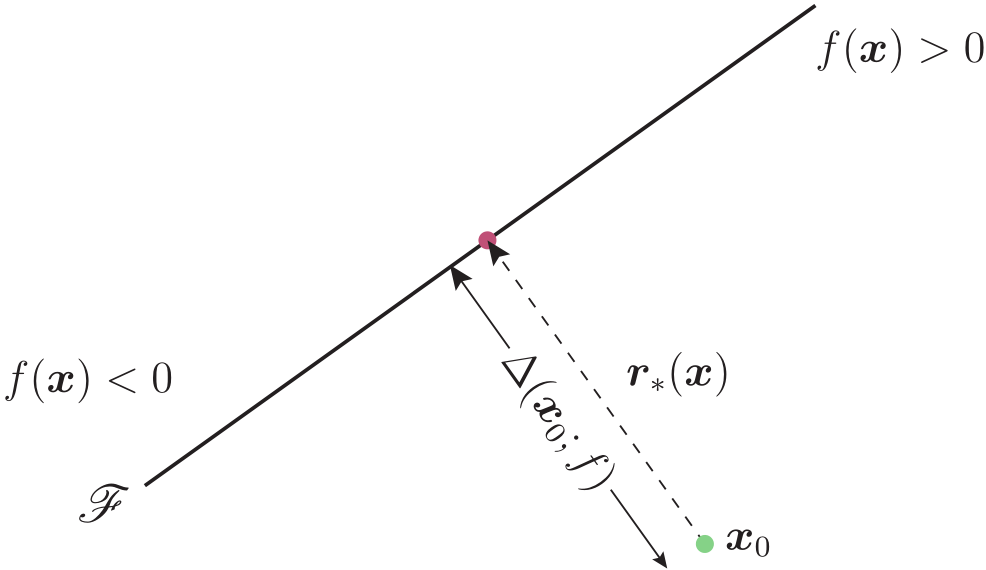
\includegraphics[width=0.3\textwidth]{docs/paperReading/deepfool/deepfool-adv_example_in_linear_classifier.png}
        \end{figure}

        仿射分类器 $f(x)=\omega^T x+b$ 在 $x_0$ 的鲁棒性 $\Delta(x_0;f)$ 等于从 $x_0$ 到仿射超平面 $\mathscr{F}=\{x:\omega^T x+b=0\}$ 的距离

        改变分类器决策的最小扰动 $r_*(x_0)$ 是 $x_0$ 在分类边界 
        $\mathscr{F}$ 上的正交投影:
        \begin{equation}
            \begin{aligned}
                r_*(x_0)    &:=argmin ||r||_2 \\
                            &\text{subject to } sign(f(x_0+r))\neq sign(f(x_0)) \\
                            &=-\frac{f(x_0)}{||\omega||_2^2}\omega
            \end{aligned}
        \end{equation}
    \end{multicols}
\end{frame}

\begin{frame}{对于二分类器DeepFool attack}
    \begin{multicols}{2}
        假设 $f$ 是一个通用的可微的二分类器,采用迭代程序来估计鲁棒性 $\Delta(x_0;f)$ :

        每次迭代中,$f$ 会在当前点 $x_i$ 周围被线性化,线性化分类器的最小扰动为P
        \begin{equation}
            \begin{aligned}
                & argmin_{r_i} ||r_i||_2 \\
                & \text{ subject to } f(x_i)+\nabla f(x_i)^T r_i=0
            \end{aligned}
        \end{equation}
        第 $i$ 轮迭代的扰动 $r_i$ 可以用 $r_*(x_0)$ 计算得出,并且更新下一轮的 $x_{i+1}$ ,直到 $x_{i+1}$ 的符号改变为止

        程序的算法如下:
        \begin{figure}
            \centering
            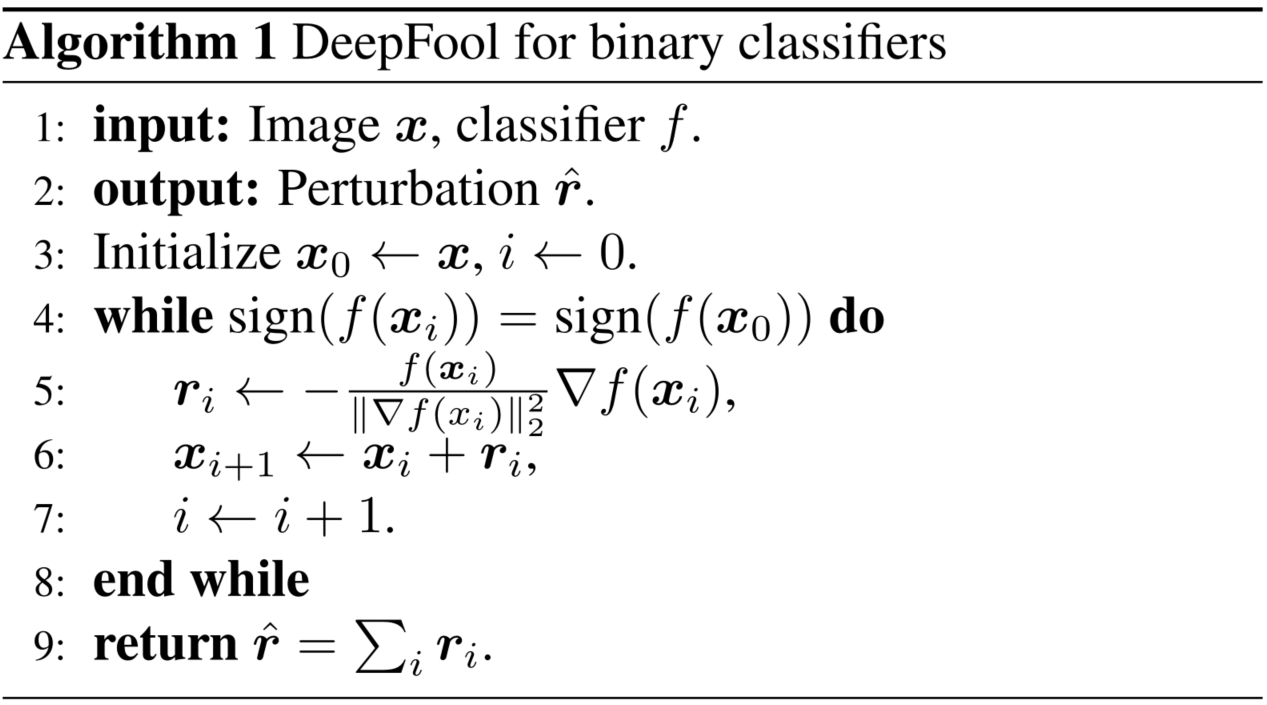
\includegraphics[width=0.7\textwidth]{docs/paperReading/deepfool/deepfool-algorithm_1.png}
        \end{figure}
    \end{multicols}
\end{frame}

\begin{frame}{对于多分类器DeepFool attack}
    多分类器有$c$个分类输出,定义为 $f:\mathbb{R}^n\rightarrow R^c$,分类通过下面映射完成
    \begin{equation}
        \begin{aligned}
            \hat{k}(x)=argmax_{k} f_k(x)
        \end{aligned}
    \end{equation}
    其中 $f_k(x)$ 是与第$k$个类相对应的 $f(x)$ 的输出

    仿射分类器$f(x)$对于给定的$W$和$b$有$f(x)=W^Tx+b$,映射$\hat{k}$是“一对多”的分类,欺骗分类器的最小扰动可以重写为
    \begin{equation}
        \begin{aligned}
            & argmin_{r} ||r||_2 \\
            & \text{s.t. } \exists k:\omega_k^T (x_0+r)+b_k\geq \omega_{\hat{k}(x_0)}^T(x_0+r)+b_{\hat{k}}(x_0)
        \end{aligned}
    \end{equation}
    $\omega_k$ 是$W$的第$k$列。要改变分类结果,必须保证存在一个非原始类标的分类器结果大于原始分类函数的结果
\end{frame}



\begin{frame}{对于多分类器DeepFool attack}
    \begin{multicols}{2}
        多面体 $P$ 定义了输出标签$\hat{k}(x_0)$的空间区域,$x_0$ 在凸多面体 $P$ 内部
        \begin{equation}
            \begin{aligned}
                P=\bigcap_{k=1}^c \{x:f_{\hat{k}(x_0)}(x)\geq f_k(x)\}
            \end{aligned}
        \end{equation}

        几何上,上述的问题就是计算 $x_0$ 与凸多面体 $P$ 的距离 $\textbf{dist}(x_0,P^c)$

        \begin{figure}
            \centering
            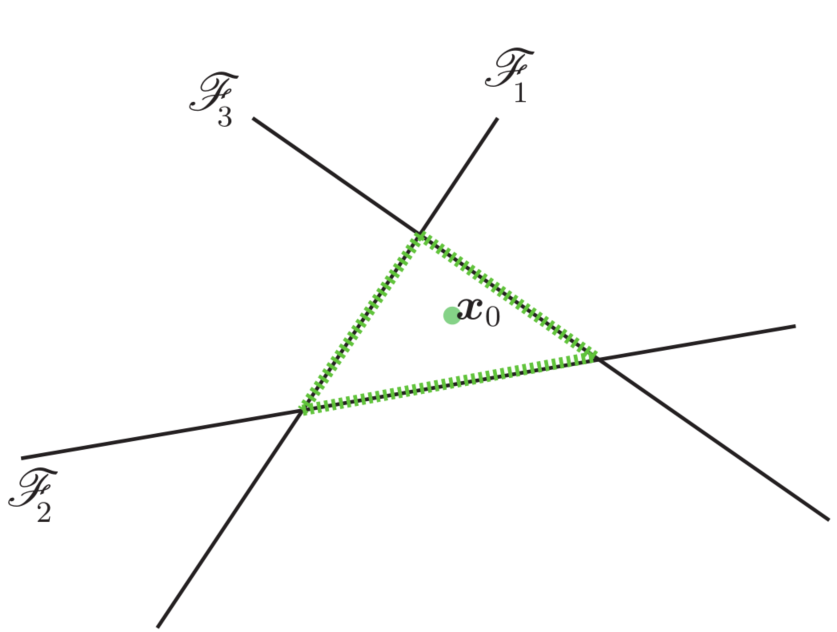
\includegraphics[width=0.3\textwidth]{docs/paperReading/deepfool/deepfool-figure4.png}
        \end{figure}

        例如属于第四类的样本$x_0$,有$\mathscr{F}_k=\{x:f_k(x)-f_4(x)=0\}$,即$x_0$不在$\mathscr{F}_1,\mathscr{F}_2,\mathscr{F}_3$任意一个超平面上。超平面用实线表示,边界$P$用绿线表示
    \end{multicols}
\end{frame}

\begin{frame}{对于多分类器DeepFool attack}
    定义$\hat{l}(x_0)$是距离边界$P$最近的超平面,图中为$\hat{l}(x_0)=3$,$\hat{l}(x_0)$可以计算为
    \begin{equation}
        \begin{aligned}
            \hat{l}(x_0)=argmin_{k\neq \hat{k}(x_0)}\frac{f_k(x_0)-f_{\hat{k}(x_0)}(x_0)}{||\omega_k-\omega_{\hat{k}(x_0)}||_2}
        \end{aligned}
    \end{equation}
    
    最小扰动距离为
    \begin{equation}
        \begin{aligned}
            r_*(x_0)=
            \frac{|f_{\hat{l}(x_0)}(x_0)-f_{\hat{k}(x_0)}(x_0)|}
            {||\omega_{\hat{l}(x_0)}-\omega_{\hat{\hat{k}(x_0)}}||_2^2}  
            (\omega_{\hat{l}(x_0)}-\omega_{\hat{k}(x_0)})
        \end{aligned}
    \end{equation}
    
    也就是说,我们找到了$x_0$在$P$上的最近投影。并且迭代算法也变成
    \begin{equation}
        \begin{aligned}
            P=\bigcap_{k=1}^c 
            \{x:f_{_k}(x_i)-f_{\hat{k}(x_0)}(x_i)+\nabla f_k(x_i)^Tx-\nabla f_{\hat{k}(x_0)}(x_i)^Tx\leq 0\}
        \end{aligned}
    \end{equation}
\end{frame}

\begin{frame}{对于多分类器DeepFool attack}
    程序的算法如下
    \begin{figure}
        \centering
        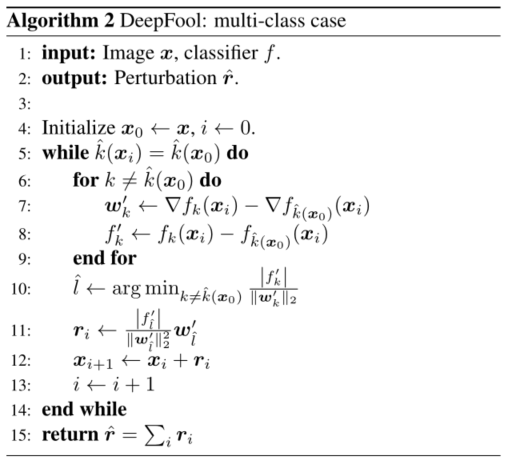
\includegraphics[width=0.46\textwidth]{docs/paperReading/deepfool/deepfool-algorithm_2.png}
    \end{figure}
\end{frame}
\begin{frame}{DeepFool attack实验结果}
    \begin{figure}
        \centering
        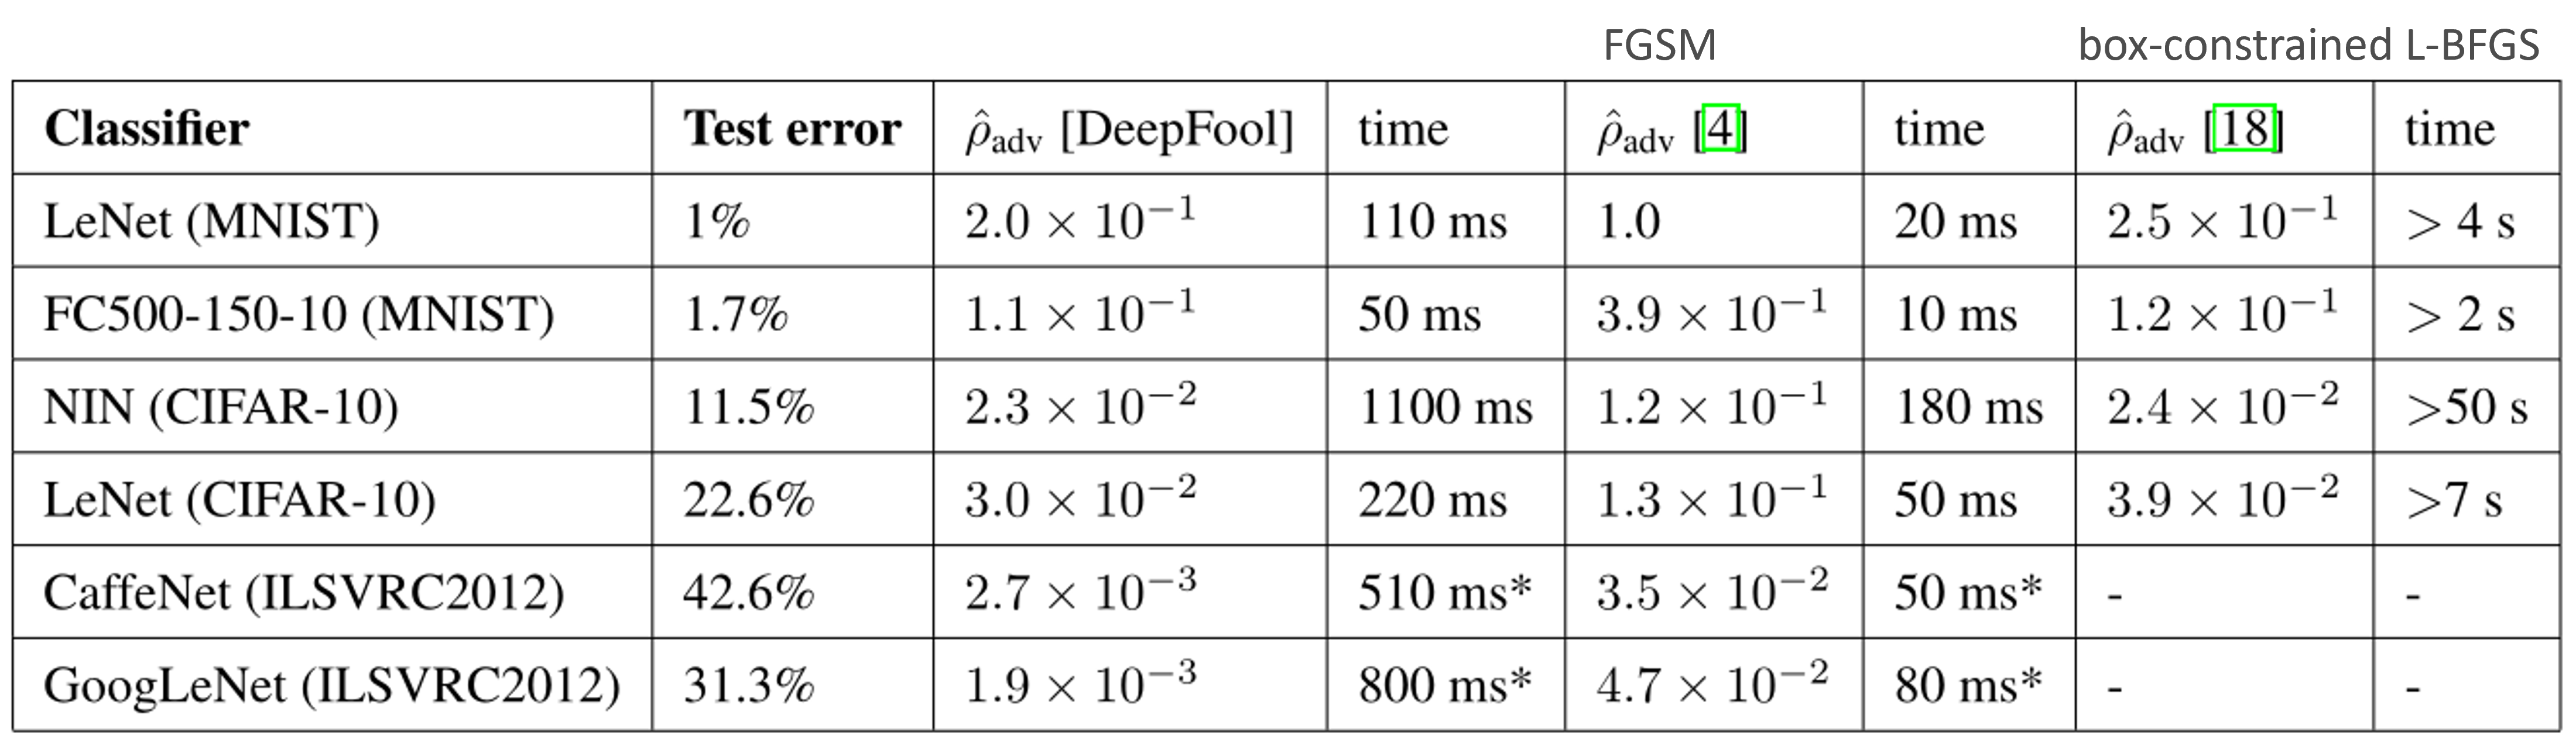
\includegraphics[width=0.9\textwidth]{docs/paperReading/deepfool/deepfool-result_1.png}
    \end{figure}
\end{frame}

\begin{frame}{DeepFool attack}
    \begin{figure}
        \centering
        \includegraphics[width=0.9\textwidth]{docs/paperReading/deepfool/deepfool-exp.png}
    \end{figure}
\end{frame}
% ----------------------------------------


% ----------------------------------------
% 2021
% \section{Experiment}

\begin{frame}{实验}
    \begin{scriptsize}
        \begin{figure}
            \centering
            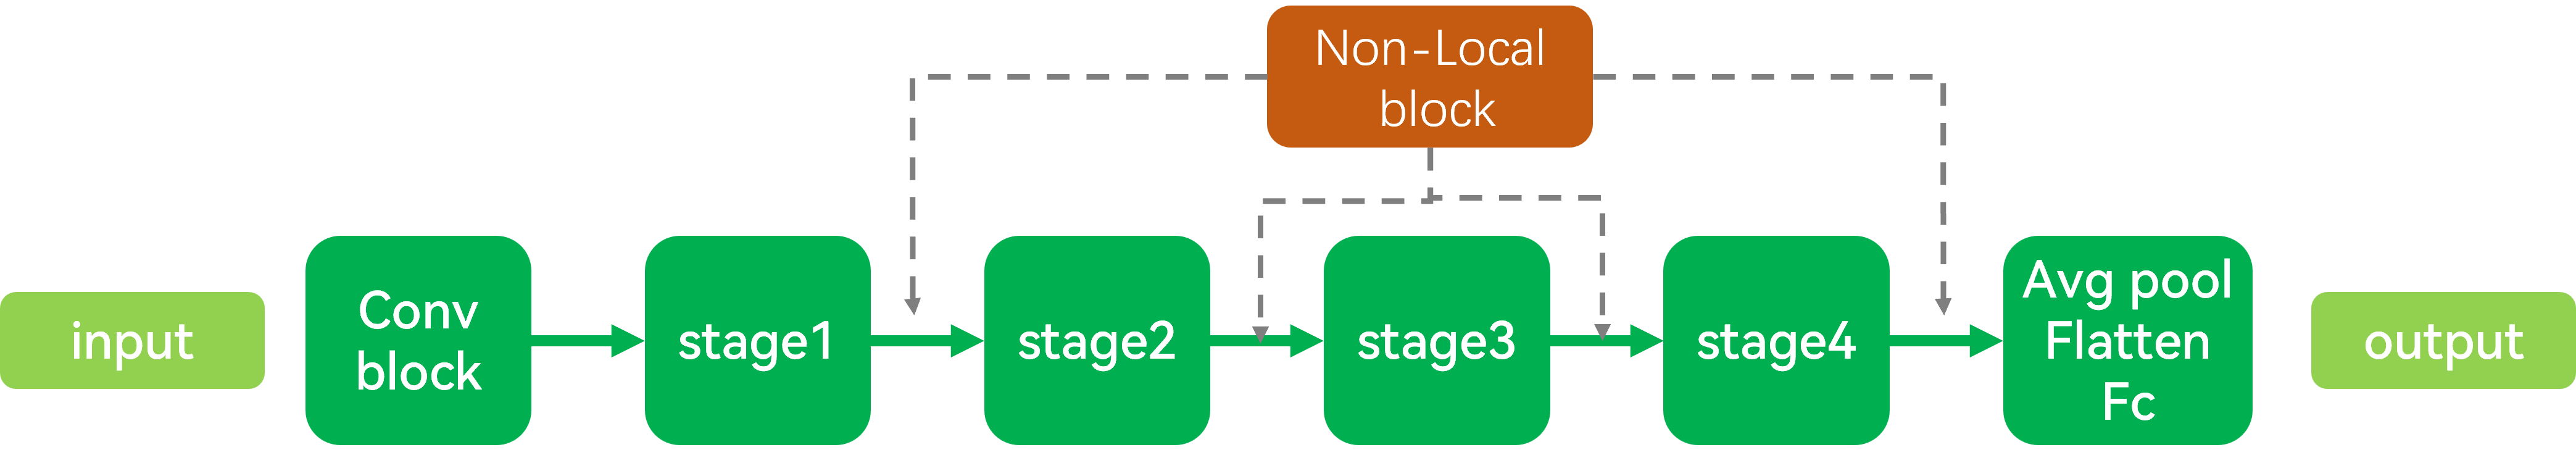
\includegraphics[width=0.9\textwidth]{docs/0903/images/resnet-nonlocal.png}
        \end{figure}
        Baseline选择ResNet-50,不同stage加入non-local模块,进行对抗训练
        \begin{table}
            \begin{tabular}{ccc}
                \hline
                模型 & 干净样本训练 & 对抗训练(FGSM生成对抗样本) \\  
                \hline          
                ResNet-50                       & 0.9380 & 0.9325 \\
                ResNet-50(Non-Local in layer-1) & 0.9365 & 0.9275 \\
                ResNet-50(Non-Local in layer-2) & 0.9420 & 0.9285 \\
                ResNet-50(Non-Local in layer-3) & 0.9455 & 0.9145 \\
                ResNet-50(Non-Local in layer-4) & 0.9310 & 0.9035 \\
                \hline          
            \end{tabular}
        \end{table}
        
        问题:模型训练的时候,在不同epoch的结果不一样,那么一些论文中的结果是怎么确定的呢?并且数据的差异很小,0.**的差异
    \end{scriptsize}    
\end{frame}

\begin{frame}{实验}
    % \begin{figure}
    %     \centering
    %     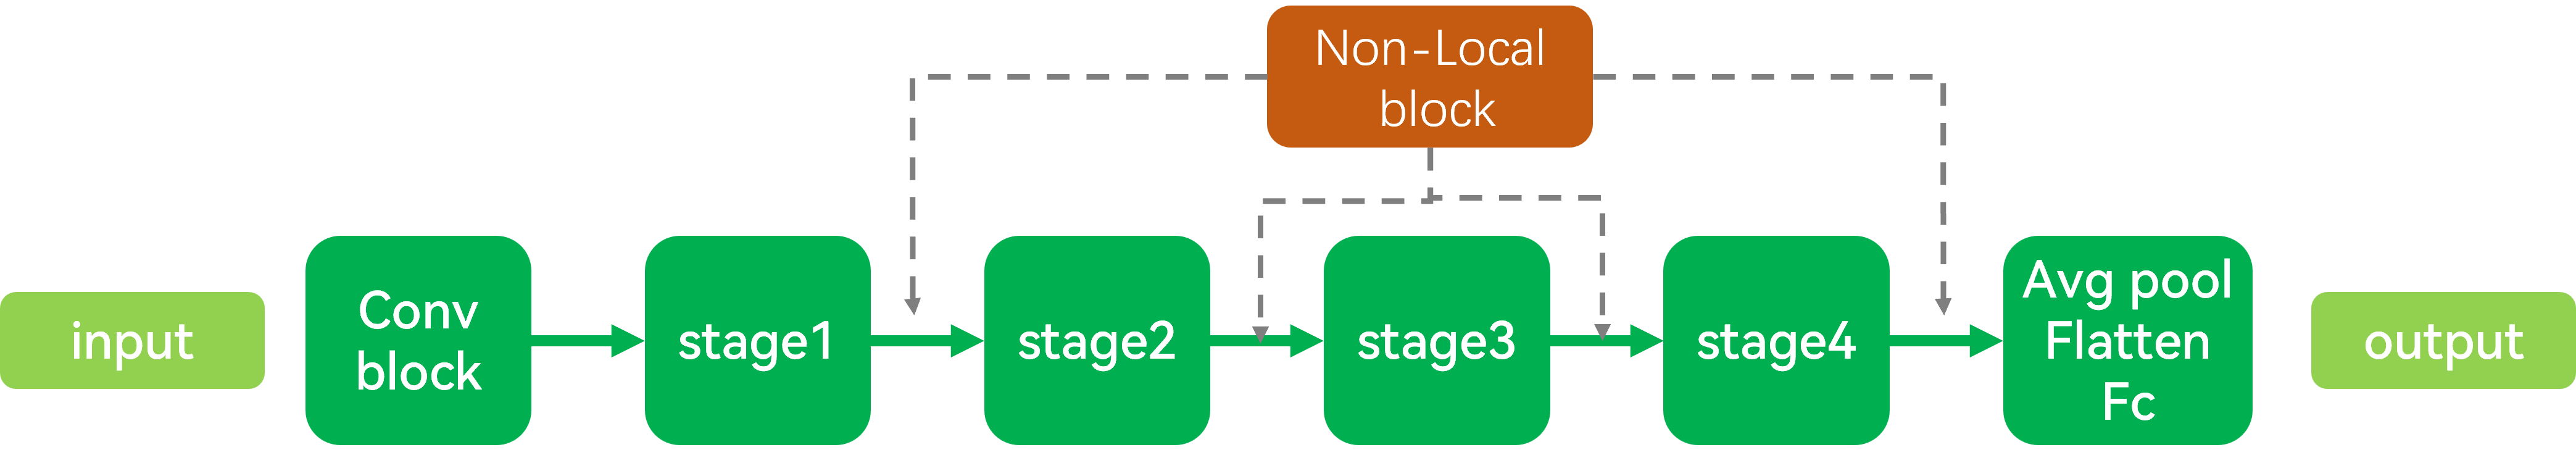
\includegraphics[width=0.7\textwidth]{docs/0903/images/resnet-nonlocal.png}
    % \end{figure}

    在模型微调的时候,如果想在模型中加入不同的模块验证他们的作用(消融实验?),在自己训练完成之后的模型(ResNet50)有BN层参数,但是加载模型库里面的模型没有BN层,那这个时候会不会对结果有影响之类的(好像没有办法把这些训练好的BN层的参数加载到新的模型上)
    \begin{figure}
        \centering
        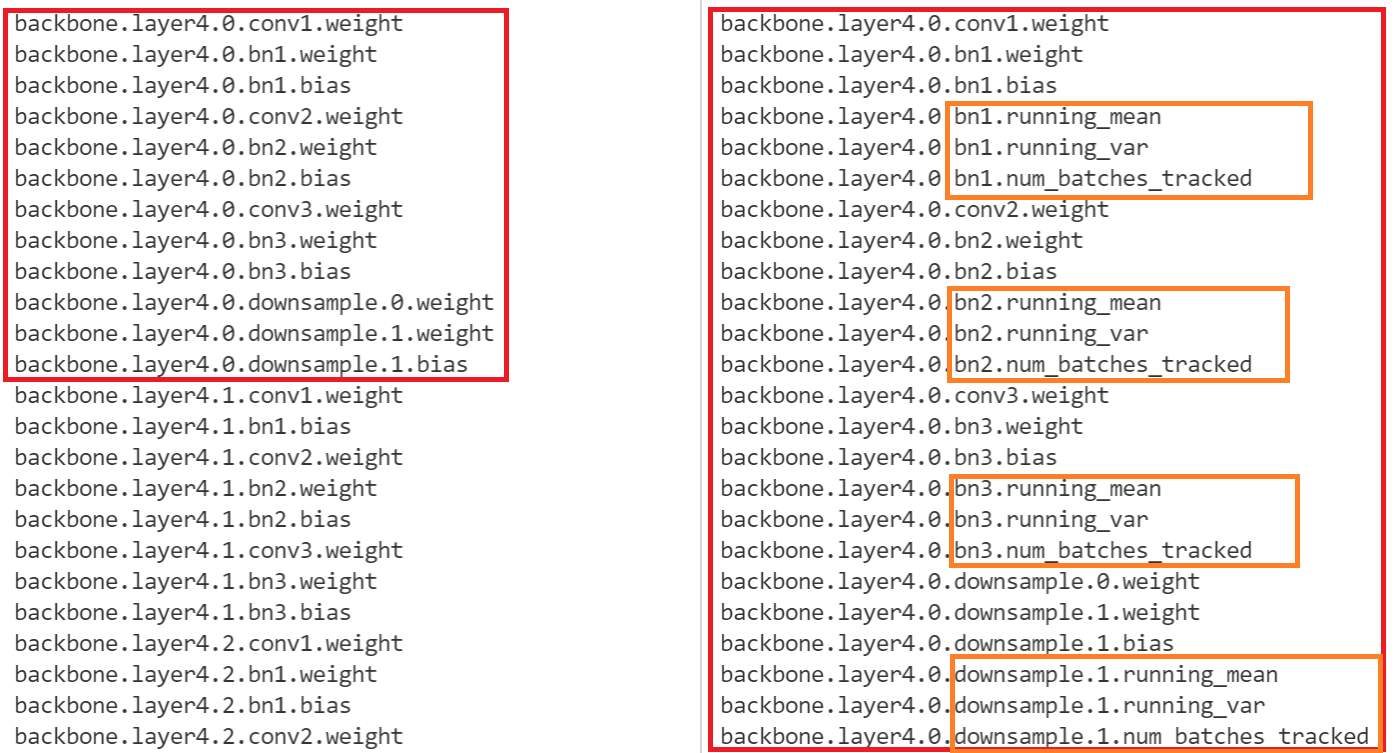
\includegraphics[width=0.6\textwidth]{docs/0903/images/s.png}
    \end{figure}
\end{frame}
% \section{Experiment}

\begin{frame}{实验}
    \begin{scriptsize}
        \begin{figure}
            \centering
            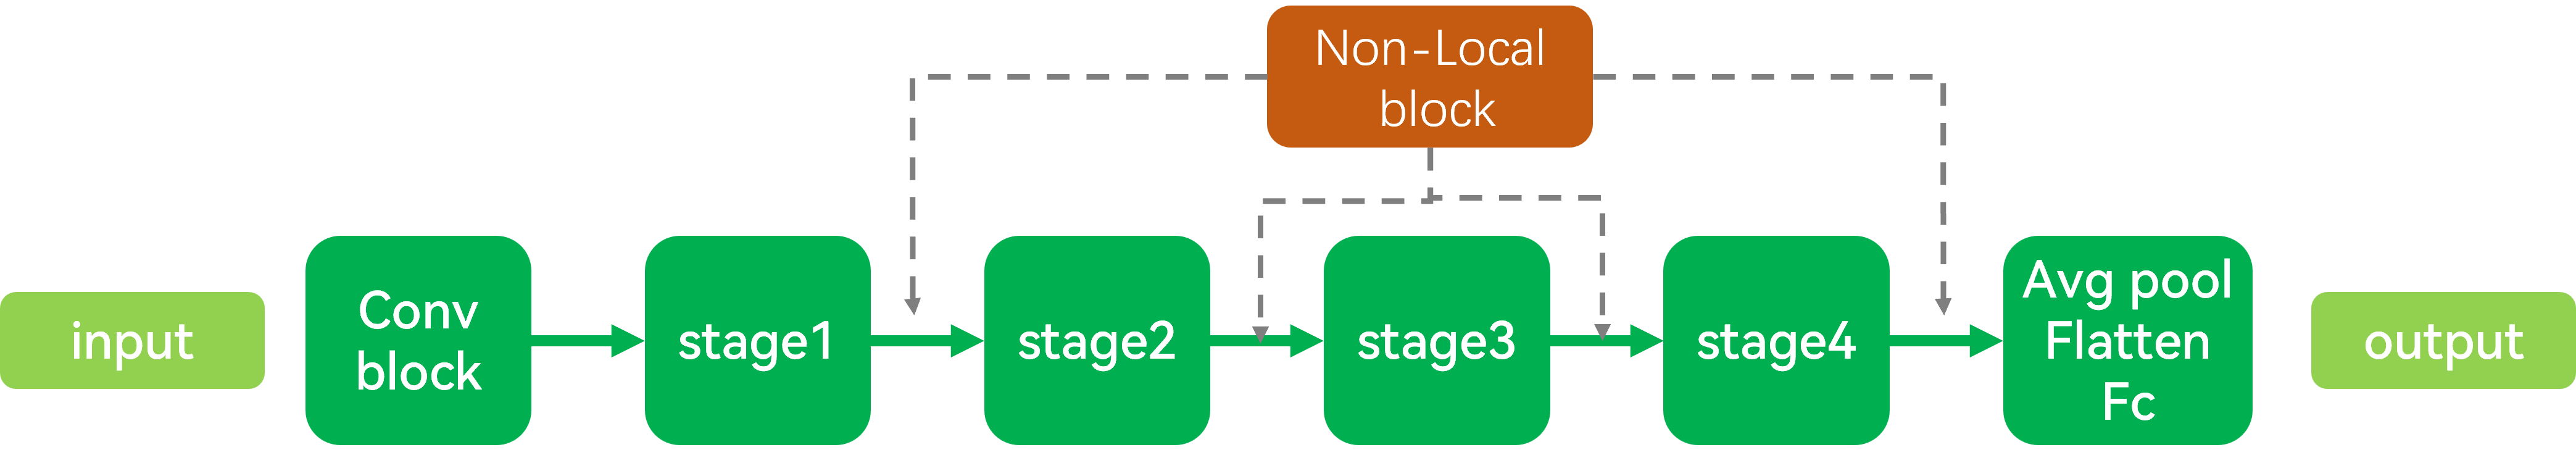
\includegraphics[width=0.9\textwidth]{docs/0903/images/resnet-nonlocal.png}
        \end{figure}
        Baseline选择ResNet-50,不同stage加入non-local模块,进行对抗训练
        \begin{table}
            \begin{tabular}{ccc}
                \hline
                模型 & 干净样本训练 & 对抗训练(FGSM生成对抗样本) \\  
                \hline          
                ResNet-50                       & 0.9380 & 0.9325 \\
                ResNet-50(Non-Local in layer-1) & 0.9365 & 0.9275 \\
                ResNet-50(Non-Local in layer-2) & 0.9420 & 0.9285 \\
                ResNet-50(Non-Local in layer-3) & 0.9455 & 0.9145 \\
                ResNet-50(Non-Local in layer-4) & 0.9310 & 0.9035 \\
                \hline          
            \end{tabular}
        \end{table}
        
        问题:模型训练的时候,在不同epoch的结果不一样,那么一些论文中的结果是怎么确定的呢?并且数据的差异很小,0.**的差异
    \end{scriptsize}    
\end{frame}

\begin{frame}{实验}
    % \begin{figure}
    %     \centering
    %     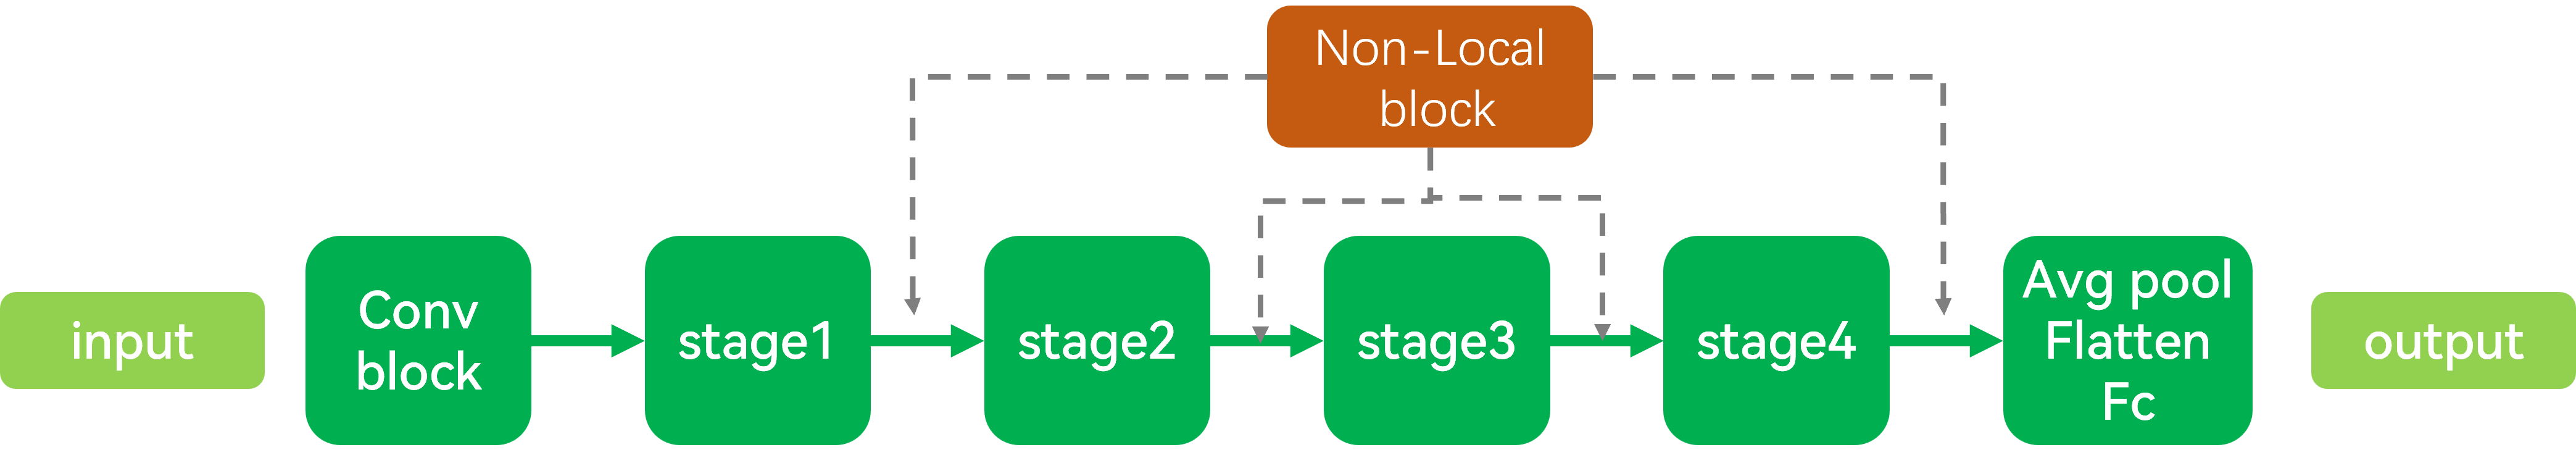
\includegraphics[width=0.7\textwidth]{docs/0903/images/resnet-nonlocal.png}
    % \end{figure}

    在模型微调的时候,如果想在模型中加入不同的模块验证他们的作用(消融实验?),在自己训练完成之后的模型(ResNet50)有BN层参数,但是加载模型库里面的模型没有BN层,那这个时候会不会对结果有影响之类的(好像没有办法把这些训练好的BN层的参数加载到新的模型上)
    \begin{figure}
        \centering
        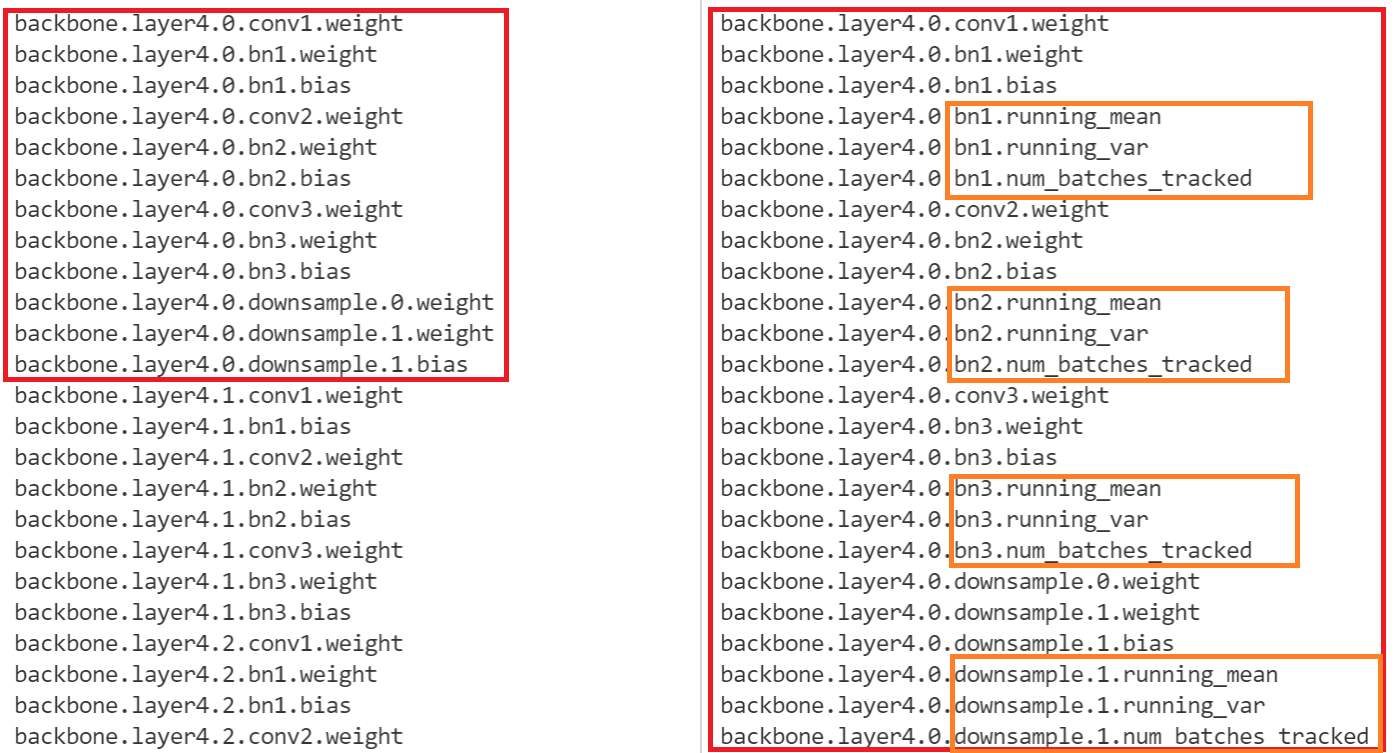
\includegraphics[width=0.6\textwidth]{docs/0903/images/s.png}
    \end{figure}
\end{frame}
% \section{根据攻击策略分类:优化}


\begin{frame}{基于优化的攻击方法}
    白盒攻击
    \begin{itemize}
        \item \textbf{L-BFGS}: 有目标攻击, Intriguing properties of neural networks
        \item \textbf{DeepFool}: 无目标攻击, a simple and accurate method to fool deep neural networks
        \item \textbf{UAP}: 无目标攻击, Universal adversarial perturbations
        \item \textbf{CW}: 有/无目标攻击, Towards Evaluating the Robustness of Neural Networks
    \end{itemize}

    黑盒攻击
    \begin{itemize}
        \item \textbf{Grad.Est.}: 有/无目标攻击, Exploring the space of black-box attacks on deep neural networks
        \item \textbf{ZOO}: 有/无目标攻击, ZOO:Zeroth pder optimization based black-box attacks to deep neural networks without training substitute models.
        \item \textbf{IS}: 有/无目标攻击, Simple black-box adversarial perturbations on deep neural networks
    \end{itemize}
\end{frame}


\begin{frame}{基于优化的攻击方法}
    需要解决的含约束条件的优化问题
    \begin{equation}
        \begin{aligned}
            \textbf{Minimize }    & ||r||_2 \\
            \textbf{subject to }  & f(x+r)=l \textbf{ or } f(x+r)\neq f(x) \\
                                & x+r \in [0,1]^m
        \end{aligned}
    \end{equation}
    求解满足约束条件的最小对抗扰动 $r$ ,就可以产生对抗样本 
\end{frame}


\begin{frame}{基于优化的攻击策略}

    4种基于优化的白盒攻击 L-BFGS, CW, DeepFool, UAP
    \begin{itemize}
        \item \textbf{1. L-BFGS}: 有目标攻击
    \end{itemize}
    \begin{equation}
        \textbf{Minimize } c \cdot ||r||_2 + loss_f(x+r,l) \textbf{ subject to } x+r \in [0,1]^m
    \end{equation}
    将对抗样本$x+r$经过分类器的预测输出定向为目标标签$l$

    \begin{itemize}
        \item \textbf{2. CW}: 有目标/无目标攻击
    \end{itemize}  
    \begin{equation}
        \textbf{Minimize } ||r||_2 + c \cdot f(x+r) \textbf{ subject to } x+r \in [0,1]^m
    \end{equation}
    提出了7种目标函数 $f$ 来进行优化

    
\end{frame}

\begin{frame}{基于优化的攻击策略}
    \begin{itemize}
        \item \textbf{3. DeepFool}: 无目标攻击
    \end{itemize}    
    \begin{equation}
        \begin{aligned}
            \textbf{Minimize }  & ||r||_2 \\
            \textbf{subject to }& sign(f(x_0=r))\neq sign(f(x_0)) \\
            or                  & \exists k:\omega_k^T(x_0+r)+b_k \geq \omega_{\hat{k}(x_0)}^T(x_0+r)+b_{\hat{k}(x_0)}
        \end{aligned}
    \end{equation}



    \begin{itemize}
        \item \textbf{3. UAP}: 无目标攻击
    \end{itemize}       
    \begin{equation}
        \begin{aligned}
            & \Delta v_i \leftarrow \arg\min\limits_{r} \text{ s.t. } \hat{k}(x_i+v+r)\neq \hat{k}(x_i) \\
            & v \leftarrow \mathcal{P}_{p,\zeta}=\arg\min\limits_{v'} ||v-v'||_2 \text{ subject to } ||v'||_p\leq \zeta
        \end{aligned}
    \end{equation}
\end{frame}
\section{Paper Reading: HVS in Adversarial Example}

\begin{frame}{HVS(Human Visual System)产生对抗样本的相关论文}
    \begin{itemize}
        \item 1. \emph{The Human Visual System and Adversarial AI(2020)}: HVS对低频信息更敏感,对亮度的变化比色度的变化更敏感
        \item 2. \emph{SSIMLayer: Towards Robust Deep Representation Learning via Nonlinear Structural Similarity(2018)}: 结构相似性度量 structural similarity metric, 一个提取结构信息的神经网络模块(模仿HVS)
        \item 3. \emph{Demiguise Attack: Crafting Invisible Semantic Adversarial Perturbations with Perceptual Similarity}: 利用感知相似度(一种新的图像质量度量指标,可以模拟真实世界中光照和对比度变化)来产生扰动的黑盒攻击,使用面向hvs的图像度量来处理语义信息,以生成不可见的语义对抗扰动。可以作为一个部分融合到传统攻击方法中
    \end{itemize}
\end{frame}

\begin{frame}{HVS(Human Visual System)产生对抗样本的相关论文}
    \begin{itemize}
        \item 4. \emph{GreedyFool: Multi-Factor Imperceptibility and Its Application to Designing Black-box Adversarial Example Attack}: 根据影响人眼可感知性的因素(显著畸变(JND)、韦伯-费希纳定律、纹理掩蔽和信道调制)设计多因素度量损失产生对抗样本
        \item 5. \emph{CDAE: Color decomposition-based adversarial examples for screen devices}: 为屏幕设备设计的基于颜色分解的对抗性示例方法DAE
        \item 6. \emph{Semantic Adversarial Examples}: 语义对抗样本,约束优化问题,在HSV色彩空间上添加扰动(应该基于HVS对色度变化不敏感的特点)
        \item 7. \emph{Feature Distillation: DNN-Oriented JPEG Compression Against Adversarial Examples}: 基于图像压缩技术的抗对抗实例攻击方法
    \end{itemize}
\end{frame}

\begin{frame}{影响HVS的因素}
    \emph{The Human Visual System and Adversarial AI}
    \begin{itemize}
        \item \textbf{HVS对低频信息更敏感}
        \item \textbf{HVS对亮度的变化比色度的变化更敏感。}
    \end{itemize}

    \emph{GreedyFool: Multi-Factor Imperceptibility and Its Application to Designing Black-box Adversarial Example Attack}
    \begin{itemize}
        \item \textbf{Just Noticeable Distortion}: JND。人眼无法感受像素周围的明显低于失真阈值以下的刺激 
        \item \textbf{Weber-Fechner Law}: 一个心理物理学的观点,明显的刺激差异保持一个恒定的比率
        \item \textbf{Texture Masking}: 纹理掩膜。人眼对平滑区域像素的干扰比纹理区域的干扰更敏感(也就是对低频变化比高频变化更加敏感)
        \item \textbf{Channel Modulation}: 通道调制,人眼对颜色通道的敏感度是有差异的。对绿色最敏感,对蓝色最不敏感。
    \end{itemize}
\end{frame}











\section{Paper Reading: IQA in Adversarial Example}

\begin{frame}{IQA( Image Quality Assessment)产生对抗样本的相关论文}
    \begin{itemize}
        \item 1.\emph{Feature Distillation: DNN-Oriented JPEG Compression Against Adversarial Examples}: 基于图像压缩技术的抗对抗实例攻击方法
        \item 2.\emph{RAN4IQA: Restorative Adversarial Nets for No-Reference Image Quality Assessment}: 基于GAN的无参考IQA
        \item 3.\emph{VR IQA NET: Deep Virtual Reality Image Quality Assessment using Adversarial Learning}: 将对抗学习应用到VR IQA中
        \item 4.\emph{Generating Adversarial Examples with an Optimized Quality}: 直接利用IQA的指标来产生对抗样本
        \item 5.\emph{A Novel Rank Learning Based No-Reference Image Quality Assessment Method}
    \end{itemize}
\end{frame}



% \section{参考文献}
% \begin{frame}[allowframebreaks]
% 	\bibliography{ref}
% 	\bibliographystyle{alpha}
% \end{frame}

\begin{frame}
    \begin{center}
        {\Huge Thanks!}
    \end{center}
\end{frame}

\end{document}